\documentclass{beamer}
\usetheme{Boadilla}
\def\*#1{\mathbf{#1}}

\usepackage{amsmath}
\usepackage{amsfonts}
\usepackage{hyperref}

\usepackage{amsmath}
\DeclareMathOperator*{\argmax}{arg\,max}
\DeclareMathOperator*{\argmin}{arg\,min}

\title{Neural Ensemble Search via Bayesian Sampling}
\author{Kseniia Petrushina}
\institute{MIPT, 2024}


\begin{document}

\begin{frame}
    \titlepage
\end{frame}


\begin{frame}
    \tableofcontents
\end{frame}


\section{Motivation \& Background}
\begin{frame}{Motivation}
    \begin{block}{Neural Architecture Search}
    Automate the design of well-performing architectures for different tasks
    \end{block}
    
    \begin{block}{Neural Network Ensembles}
    \begin{itemize}
        \item NAS algorithms select only one single architecture
        \item NNE achieve an improved performance compared with a single neural network in practice
        \item NES algorithm based on RS or evolutionary algorithm requires excessive search costs
    \end{itemize}
    \end{block} 
\end{frame}

\begin{frame}{Background}
    \begin{block}{DARTS}
    \begin{figure}
        \centering
        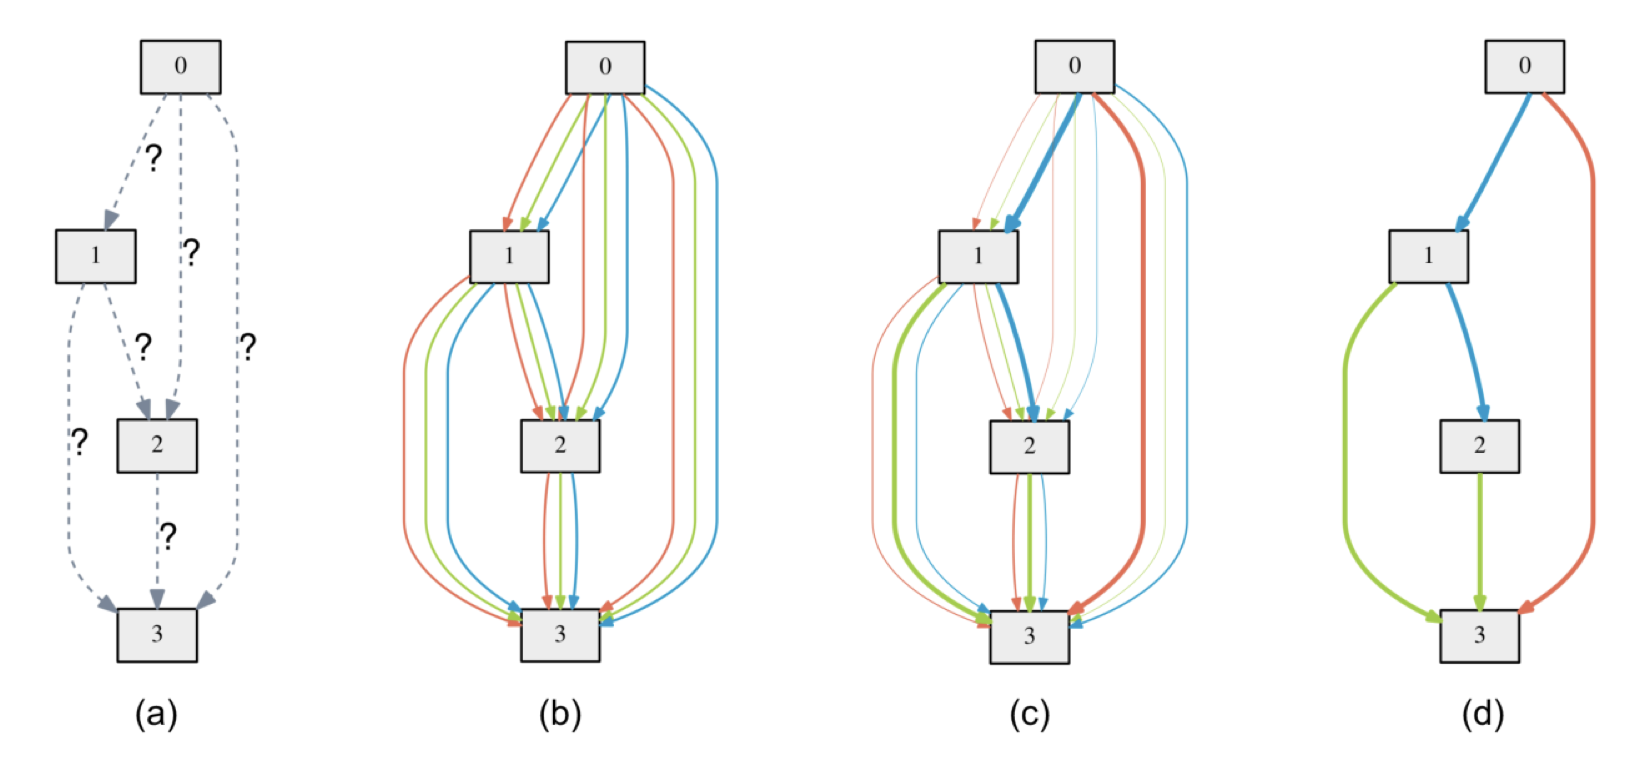
\includegraphics[width=\textwidth]{darts.png}
        \caption{(a) Unknown operations. (b) Continious relaxation of the search space. (c) Joint optimization of mixing probabilities and network weights. (d) Final architecture.}
        \label{fig:darts}
    \end{figure}
        
    \end{block}
\end{frame}

\begin{frame}{Background}

\begin{block}{Stein Variational Gradient Descent}

Approximate target distribution $p(\*x)$ with simple density $q^*(\*x) \in \mathcal{Q}$:
\[q^* = \text{arg}\min\limits_{q \in \mathcal{Q} } \{\*{KL}(q\| p) = \mathbb{E}_q [\log (q(\*x ) / p(\*x))]\}\]

$q^*(\*x)$ - set of particles $\{\*x_i\}_{i=1}^n$ iteratively updated:
\[\*x_i \leftarrow \*x_i + \varepsilon \phi^*(\*x)\]

$q_{[\varepsilon \phi]}$ - distribution of updated particles, then
\[\phi^* = \text{arg} \max_{\phi \in \mathbb{F}} \Big\{-\dfrac{d}{d\varepsilon} \*{KL} (q_{[\varepsilon \phi]} \| p) \Big|_{\varepsilon = 0} \Big\}\]
    
\end{block} 

\end{frame}

\begin{frame}{Background}
\begin{block}{Stein Variational Gradient Descent}

Closed-form solution
\[\phi^*(\cdot) = \mathbb{E}_{x\sim q} [k(\*x, \cdot) \nabla_{\*x} \log p(\*x) + \nabla_{\*x} k(\*x, \cdot)]\]

Empirical mean
\[\hat{\phi^*}(\*x_i) = \dfrac1n \sum\limits_{j=1}^n k(\*x_j, \*x_i) \nabla_{\*x_j} \log p(\*x_j) + \nabla_{\*x_j} k(\*x_j, \*x_i)\]

First term favors particles with higher probabilty dentisy, second term pushes particles away from each other
\end{block}
\end{frame}

\section{Neural Ensemble Search}

\begin{frame}{NES via Bayesian Sampling}

% \begin{equation}
Ensemble scheme
\[\mathcal{F}_S(\*x, \*\Theta^*_S)=n^{-1}\sum\limits_{\mathcal{A}\in S}\*f_A(\*x, \*\theta_A)\]
NES
\begin{gather}
 \underset{S}{\text{min}} \mathcal{L}_{\text{val}}(\mathcal{F}_S(\*x, \*\Theta^*_S)) \\
 \text{s.t. } \forall \*\theta^*_A \in \*\Theta^*_S \quad \theta^*_A = \text{arg} \min\limits_{\*\theta_A} \mathcal{L}_{\text{train}}(\*f_A(\*x, \*\theta_A)).
\end{gather}
% \end{equation}

\begin{block}{Challenges}
    \begin{enumerate}
        \item  The enormous number of candidate architectures in the NAS search space (e.g., $
        \sim 10^{25}$ in the DARTS search space)
        \item There are $\sim m^n$ different ensembles given $m$ diverse architectures
    \end{enumerate}
\end{block}

\end{frame}


\begin{frame}{Model training of supernet}

\begin{figure}
    \centering
    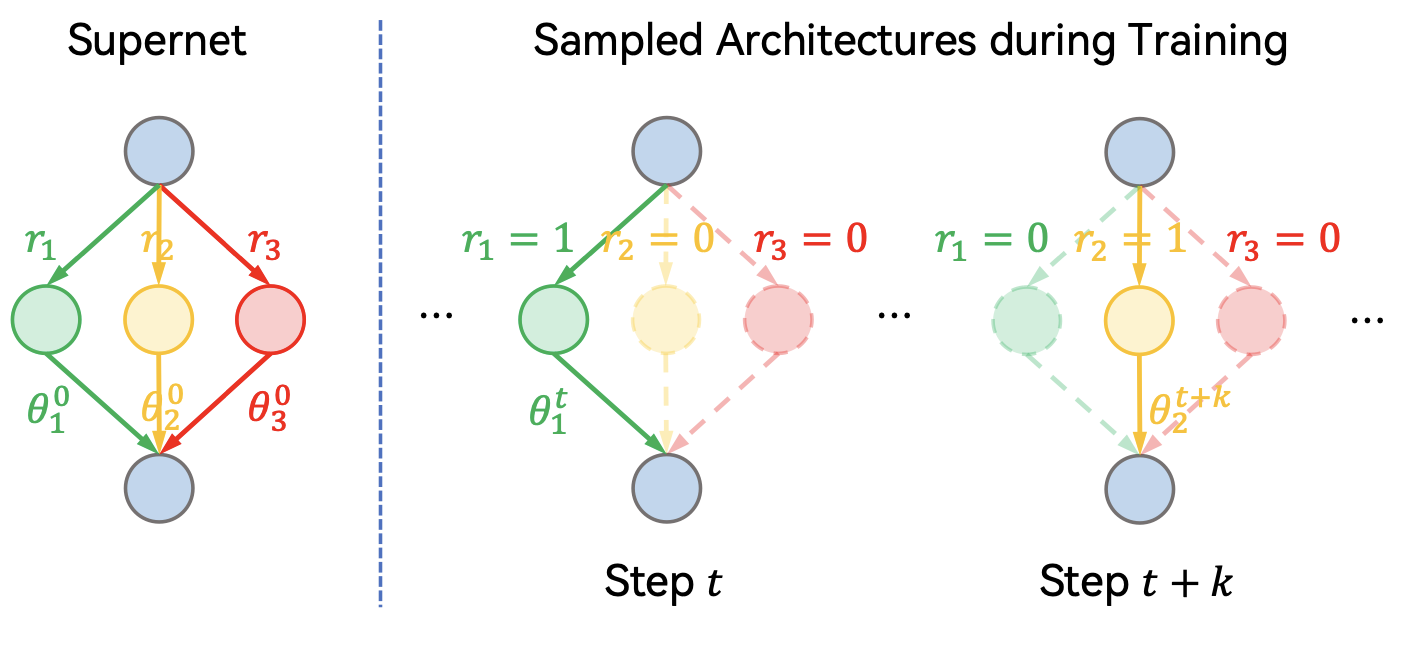
\includegraphics[width=\textwidth]{supernet.png}
    \caption{Model training of supernet. At each step only one architecture is uniformly sampled to update its parameters.}
    \label{fig:supernet}
\end{figure}
 
\end{frame}

\begin{frame}{Distribution of architectures}

\begin{block}{Single-model performance}
$\mathcal{D}$ - validation dataset, $p(\mathcal{A})$ and $p(\mathcal{A} | \mathcal{D})$ - prior and posterior distributions of a candidate architecture, $p(\mathcal{D} | \mathcal{A})$ - likelihood
\[p(\mathcal{A}| \mathcal{D}) = p(\mathcal{D} | \mathcal{A}) p(\mathcal{A}) / p(\mathcal{D}) \propto p(\mathcal{D} | \mathcal{A})\]

\end{block}

\begin{block}{Diversity}
    $\mathcal{L}(\*f)$ - $\gamma$-Lipschitz continuous loss function.
    \[\| \*f_{\mathcal{A}_1} -  \*f_{\mathcal{A}_2} \|_2 \ge \gamma^{-1} |\mathcal{L}(\*f_{\mathcal{A}_1} ) - \mathcal{L}(\*f_{\mathcal{A}_2})|\] $p(\mathcal{A}|\mathcal{D})$ can estimate diversity using $| p(\mathcal{A}_1|\mathcal{D}) - p(\mathcal{A}_2|\mathcal{D})|$
\end{block}

\begin{block}{Posterior approximation}
    Variational distribution $p_\alpha (\mathcal{A})$ approximates $p(\mathcal{A} | \mathcal{D})$:
    \begin{equation}
      \max\limits_{\*\alpha} \mathbb{E}_{\mathcal{A} \sim p_{\*\alpha}(\mathcal{A})} [\log p(\mathcal{D} | \mathcal{A})] - \*{KL}[p_{\*\alpha}(\mathcal{A}) \| p(\mathcal{A})]  
    \end{equation}

\end{block}

\end{frame}

\begin{frame}{NES via Bayesian sampling}

\begin{figure}
    \centering
    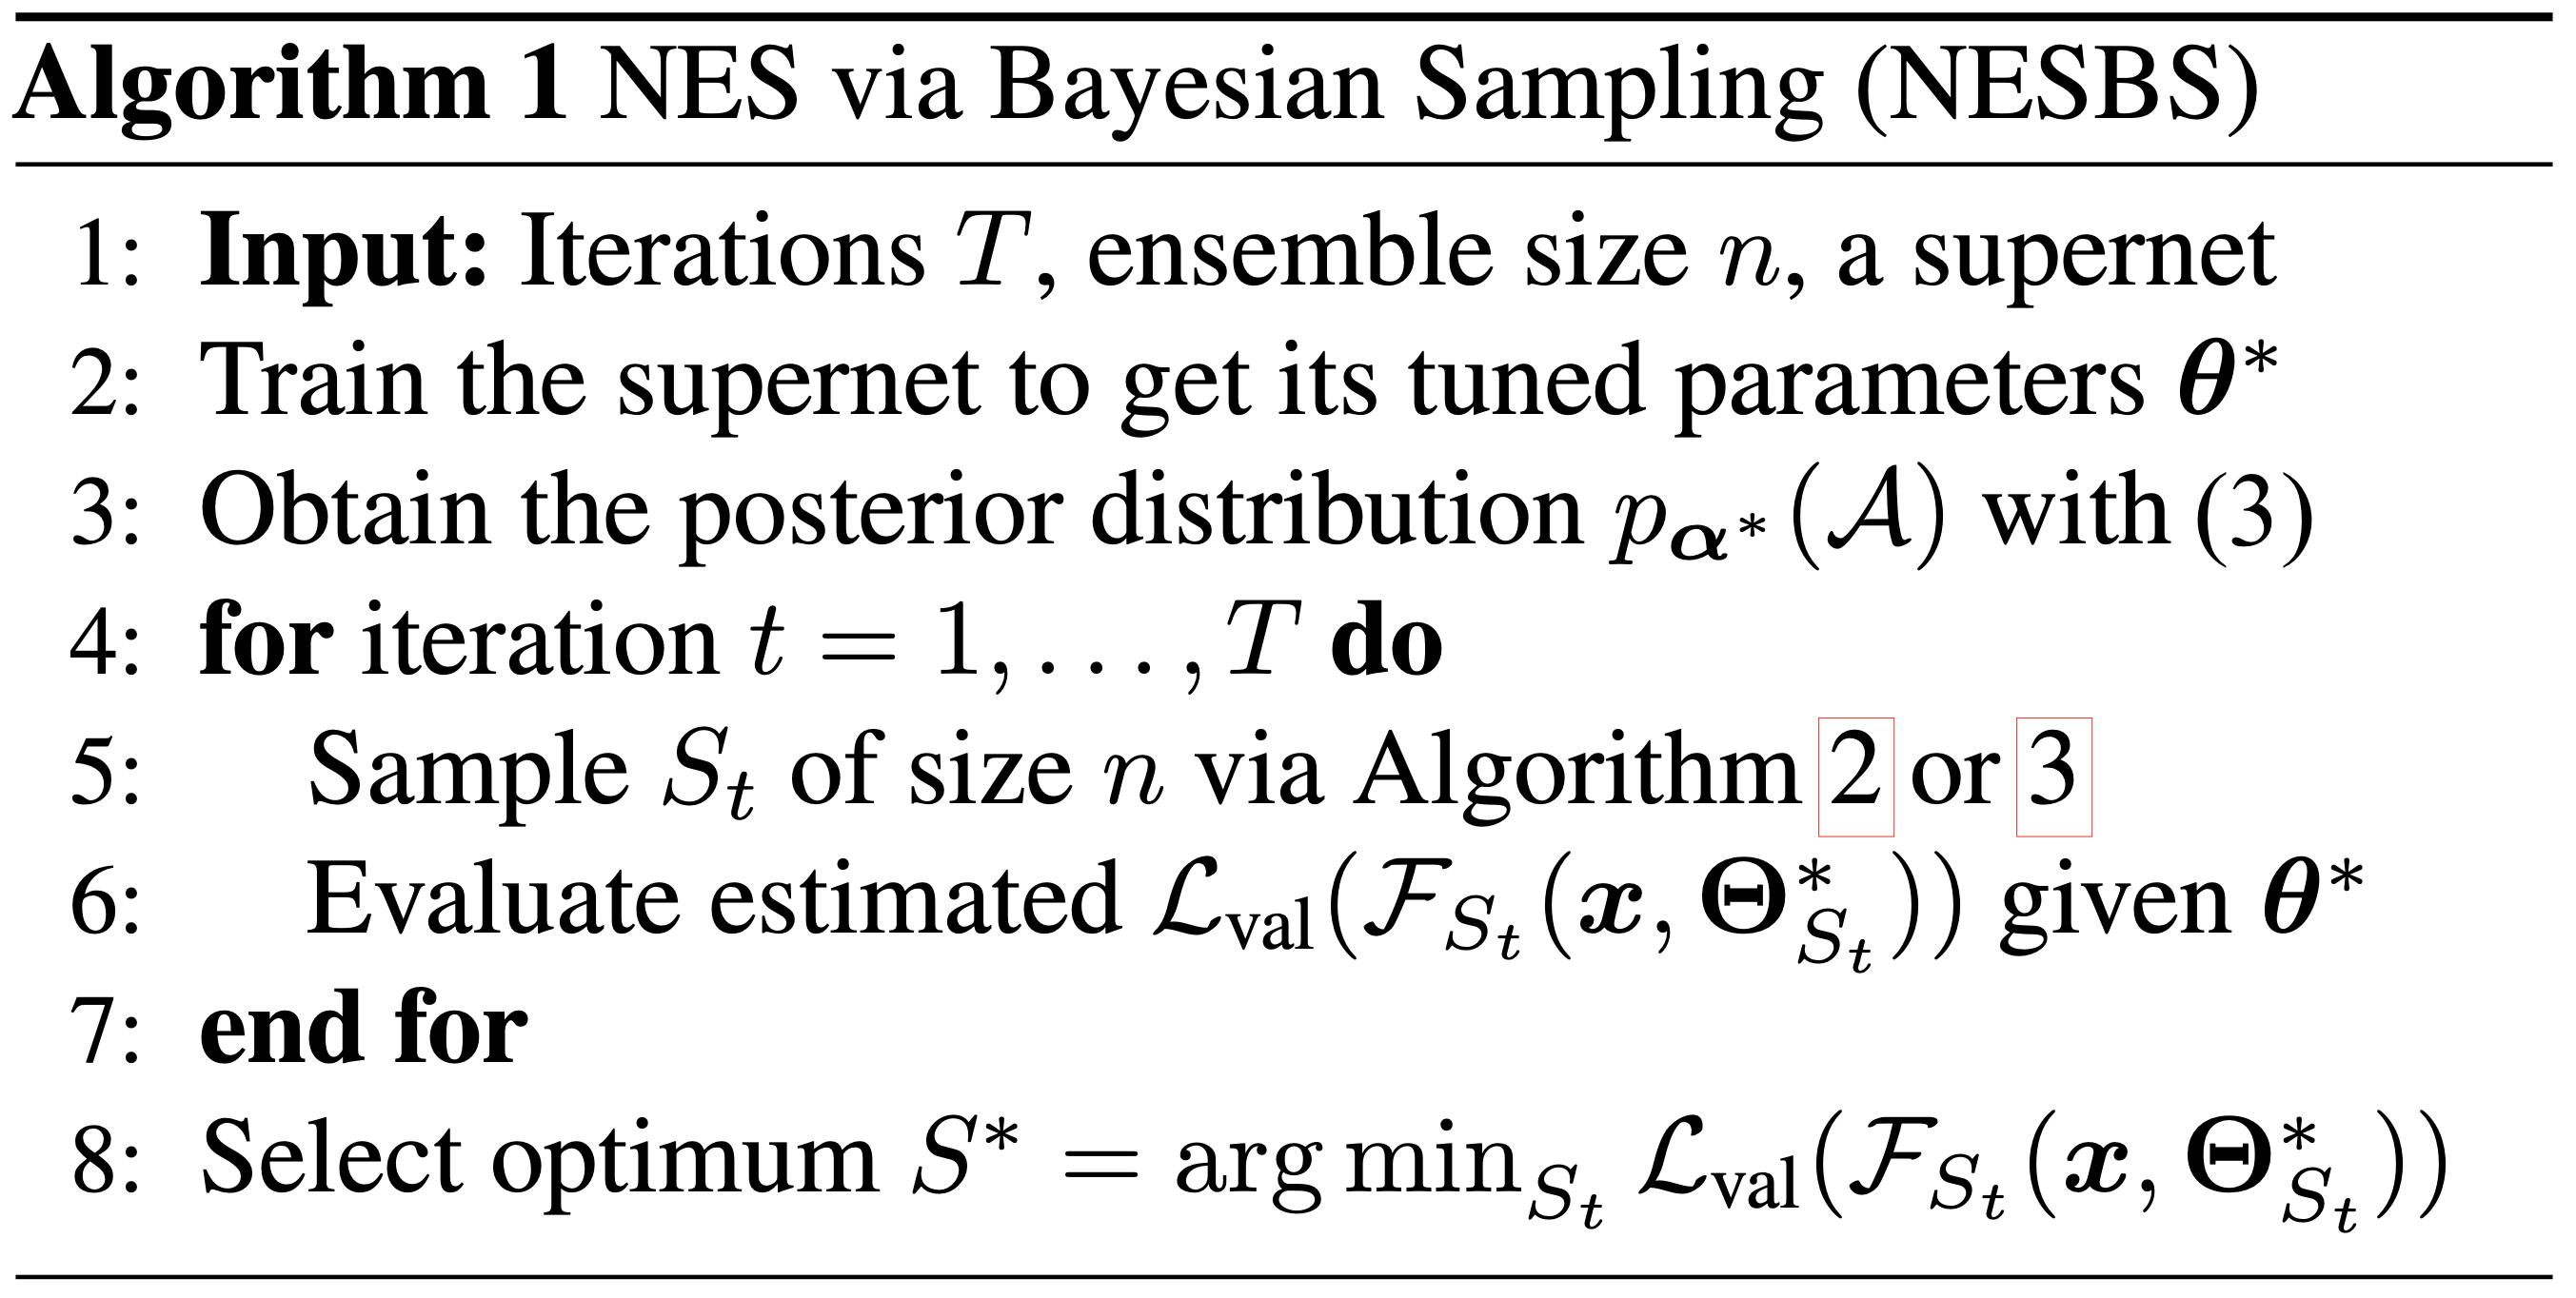
\includegraphics[width=\textwidth]{NESBS.png}
    \label{fig:nesbs}
\end{figure}

\end{frame}

\begin{frame}{Bayesian sampling}

\begin{block}{Monte-Carlo Sampling (MC)}

Sampling a set of architectures from posterior distribution
    
\end{block}

\begin{figure}
    \centering
    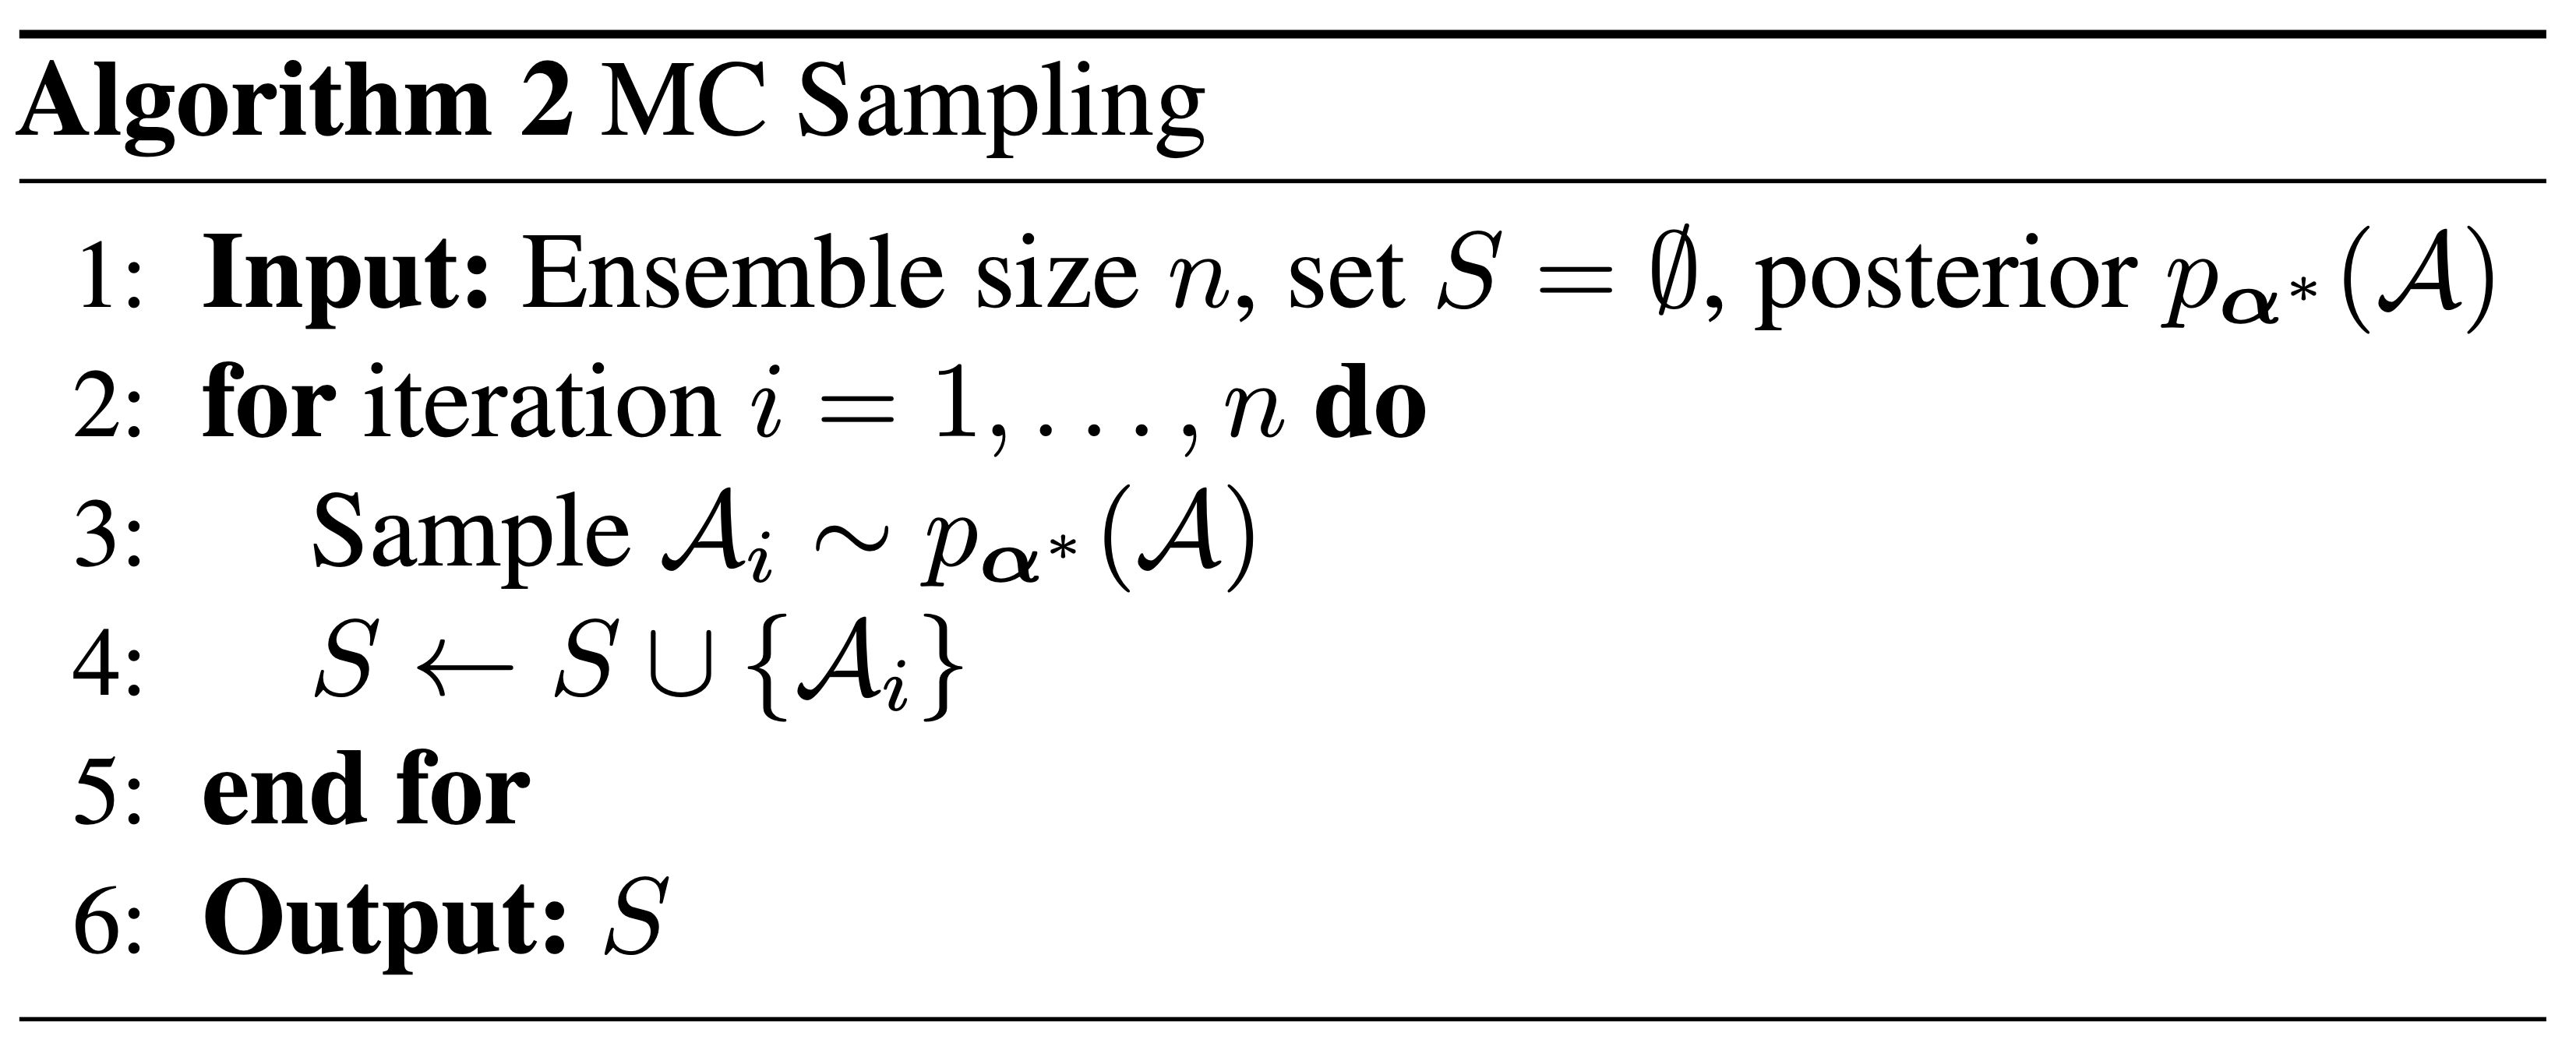
\includegraphics[width=\textwidth]{MC_BS.png}
    \label{fig:mcbs}
\end{figure}

\end{frame}

\begin{frame}{Bayesian sampling}

\begin{block}{SVGD with Regularized Diversity (RD)}
    Adding a term representing the diversity
    \[q^* = \text{arg}\min\limits_{q \in \mathcal{Q} } \{\*{KL}(q\| p)\} + n\delta \mathbb{E}_{\textbf{x}, \textbf{x}' \sim q} [k(\textbf{x}, \textbf{x}')] \]
\end{block}

\begin{figure}
    \centering
    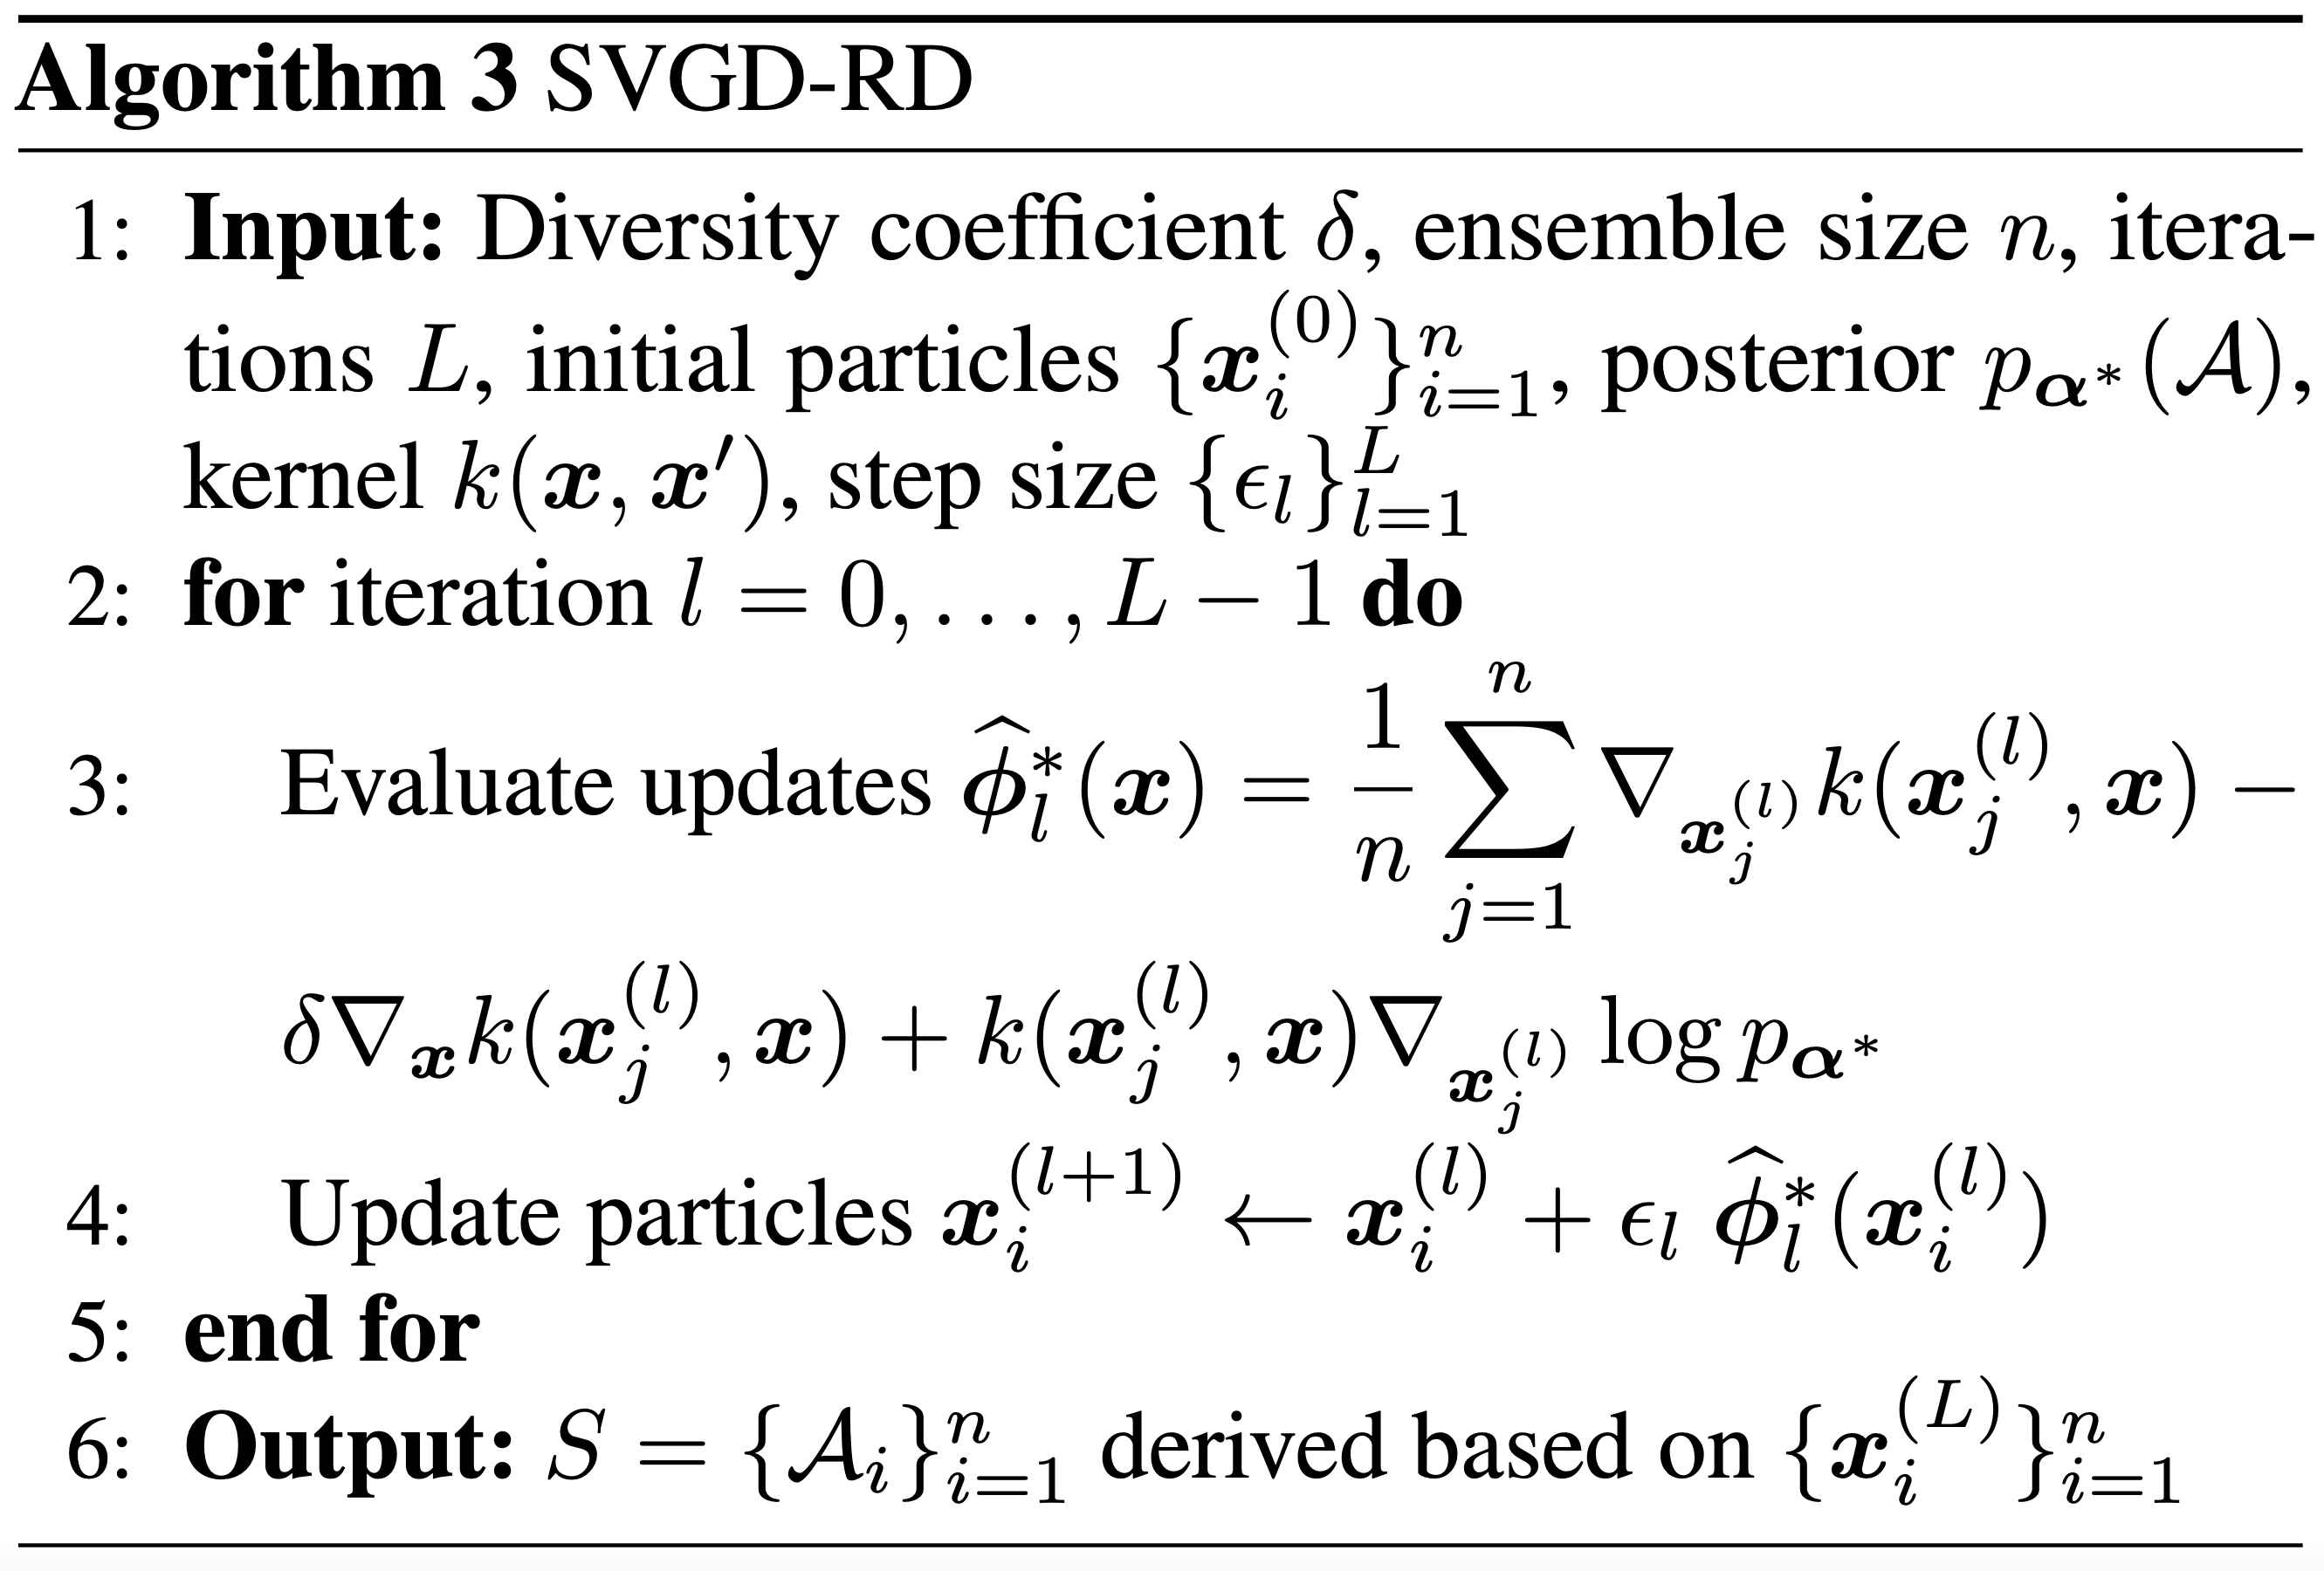
\includegraphics[width=0.7\textwidth]{SGD_BS.png}
    \label{fig:svgdbs}
\end{figure}

\end{frame}

\begin{frame}{SVGD-RD}

\begin{figure}
    \centering
    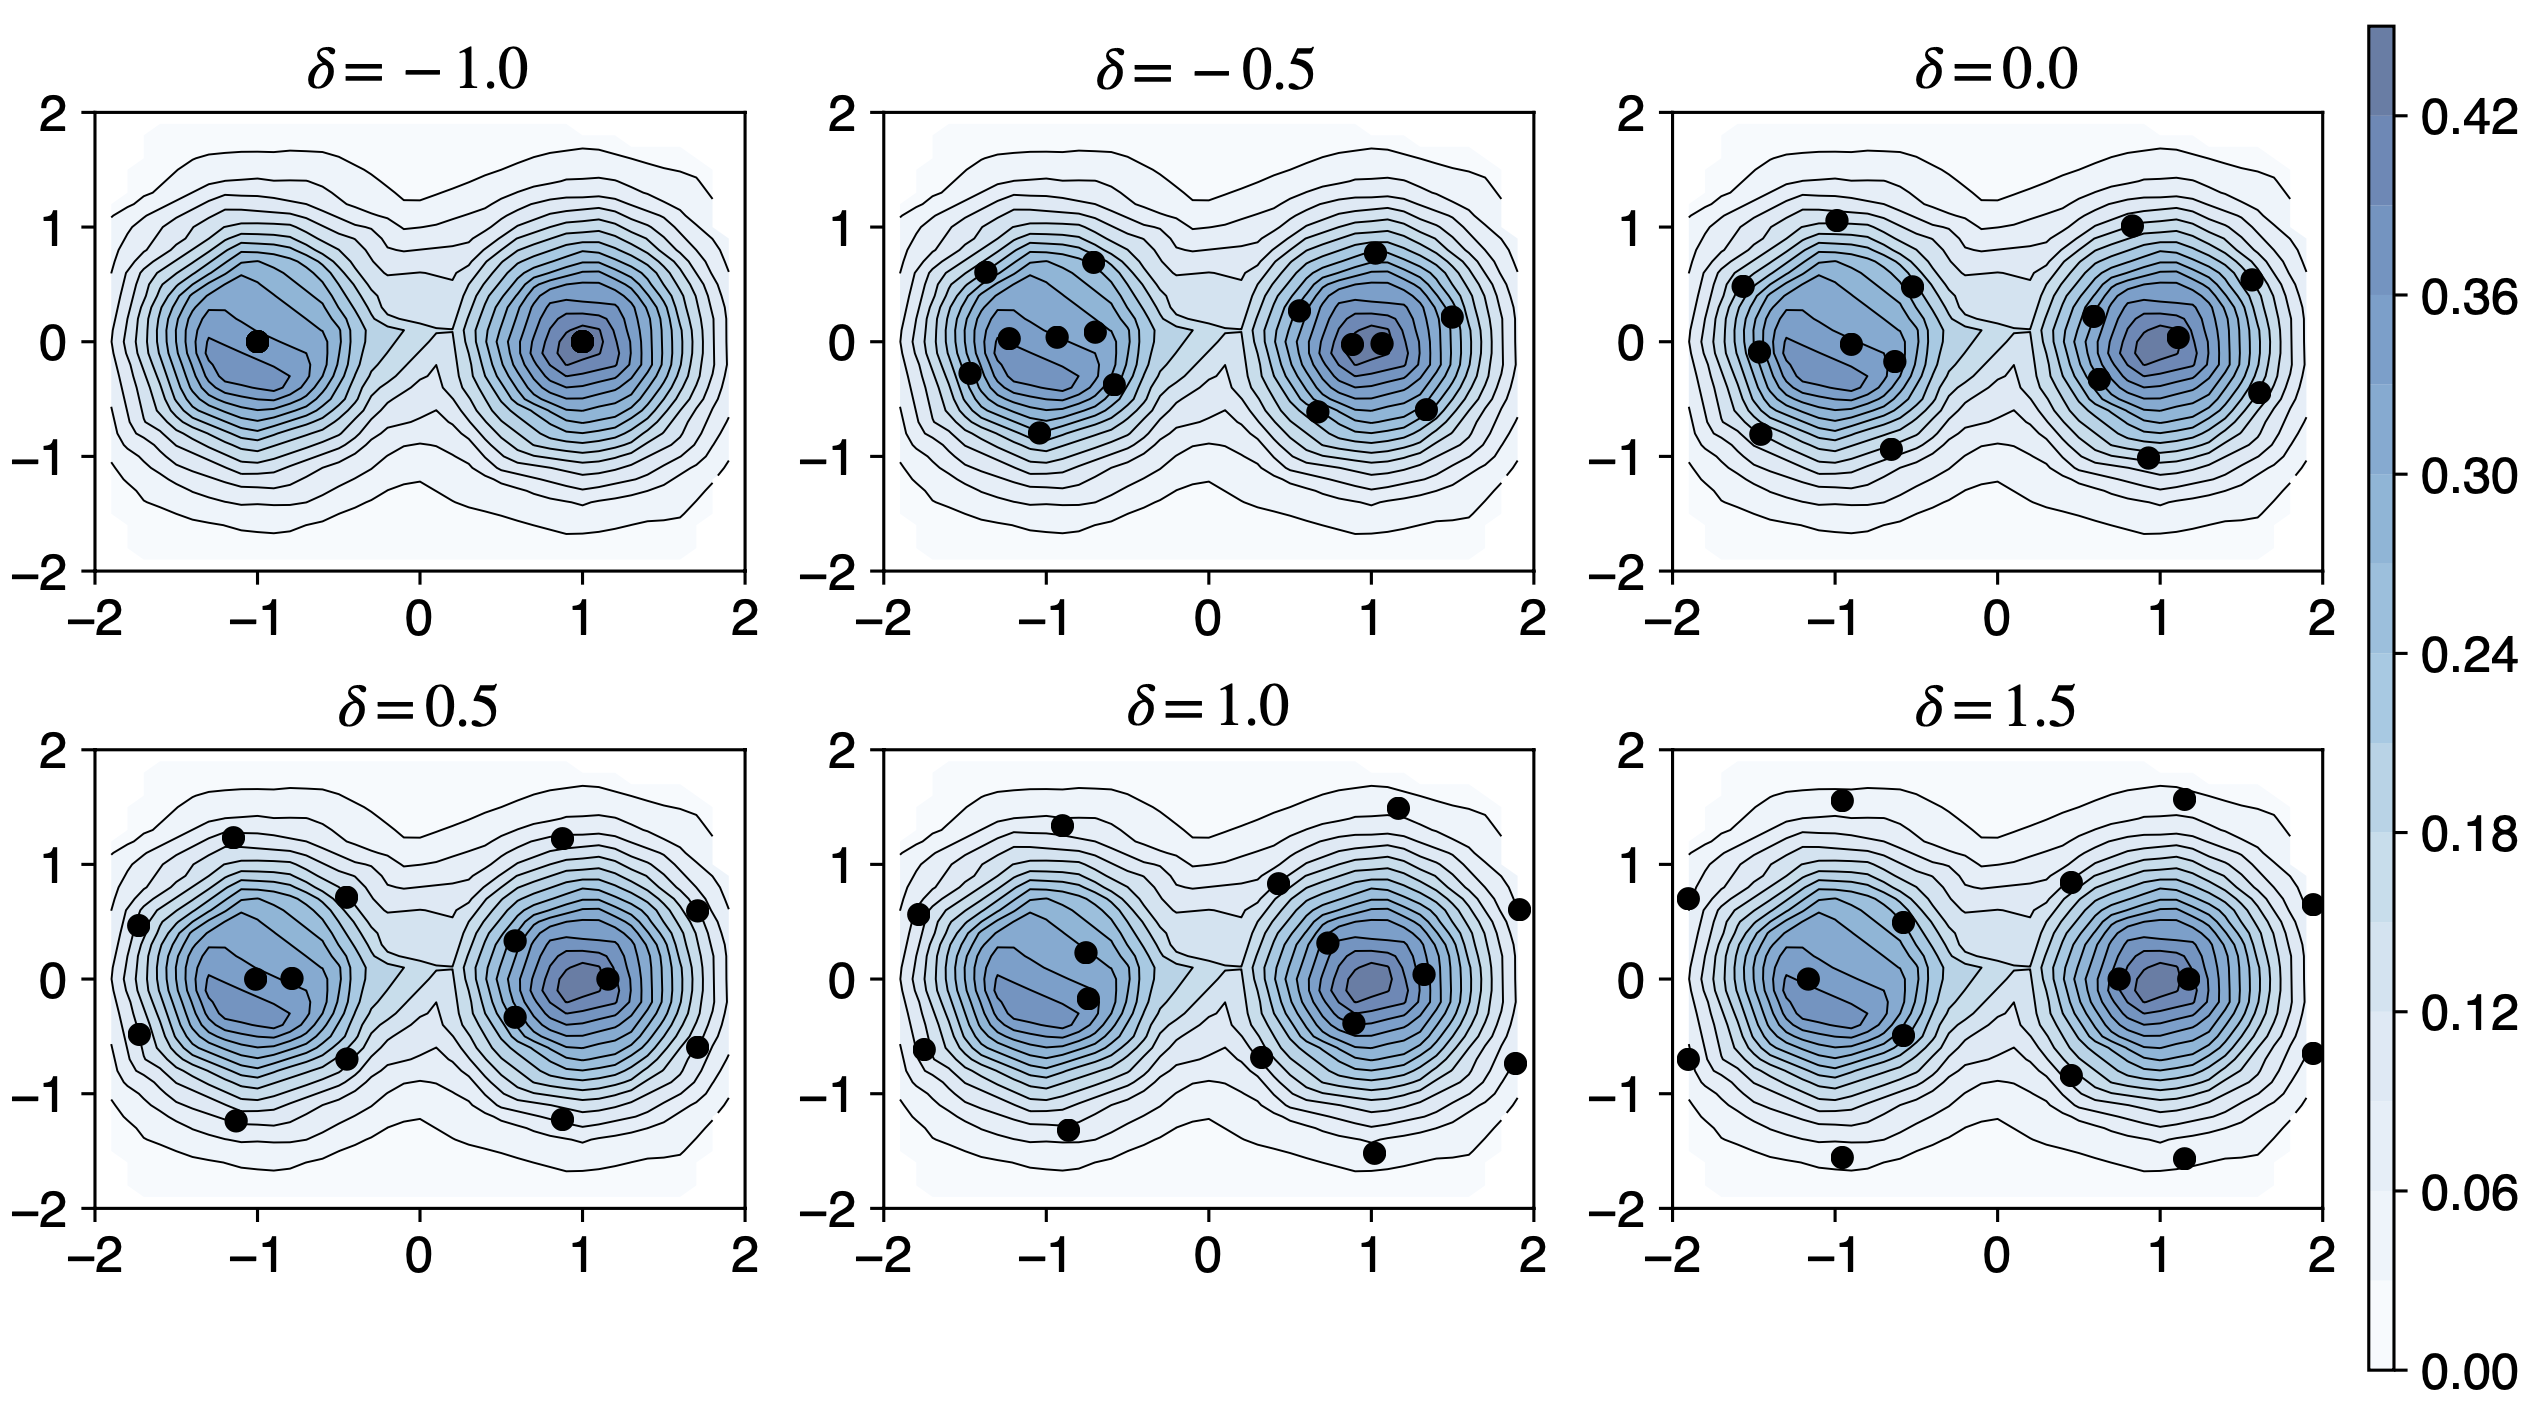
\includegraphics[width=\textwidth]{delta.png}
    \caption{Impact of $\delta$ in SVGD-RD.}
    \label{fig:delta}
\end{figure}

\end{frame}


\section{Empirical results}
\begin{frame}{Search in NAS-BENCH-201}

\begin{figure}
    \centering
    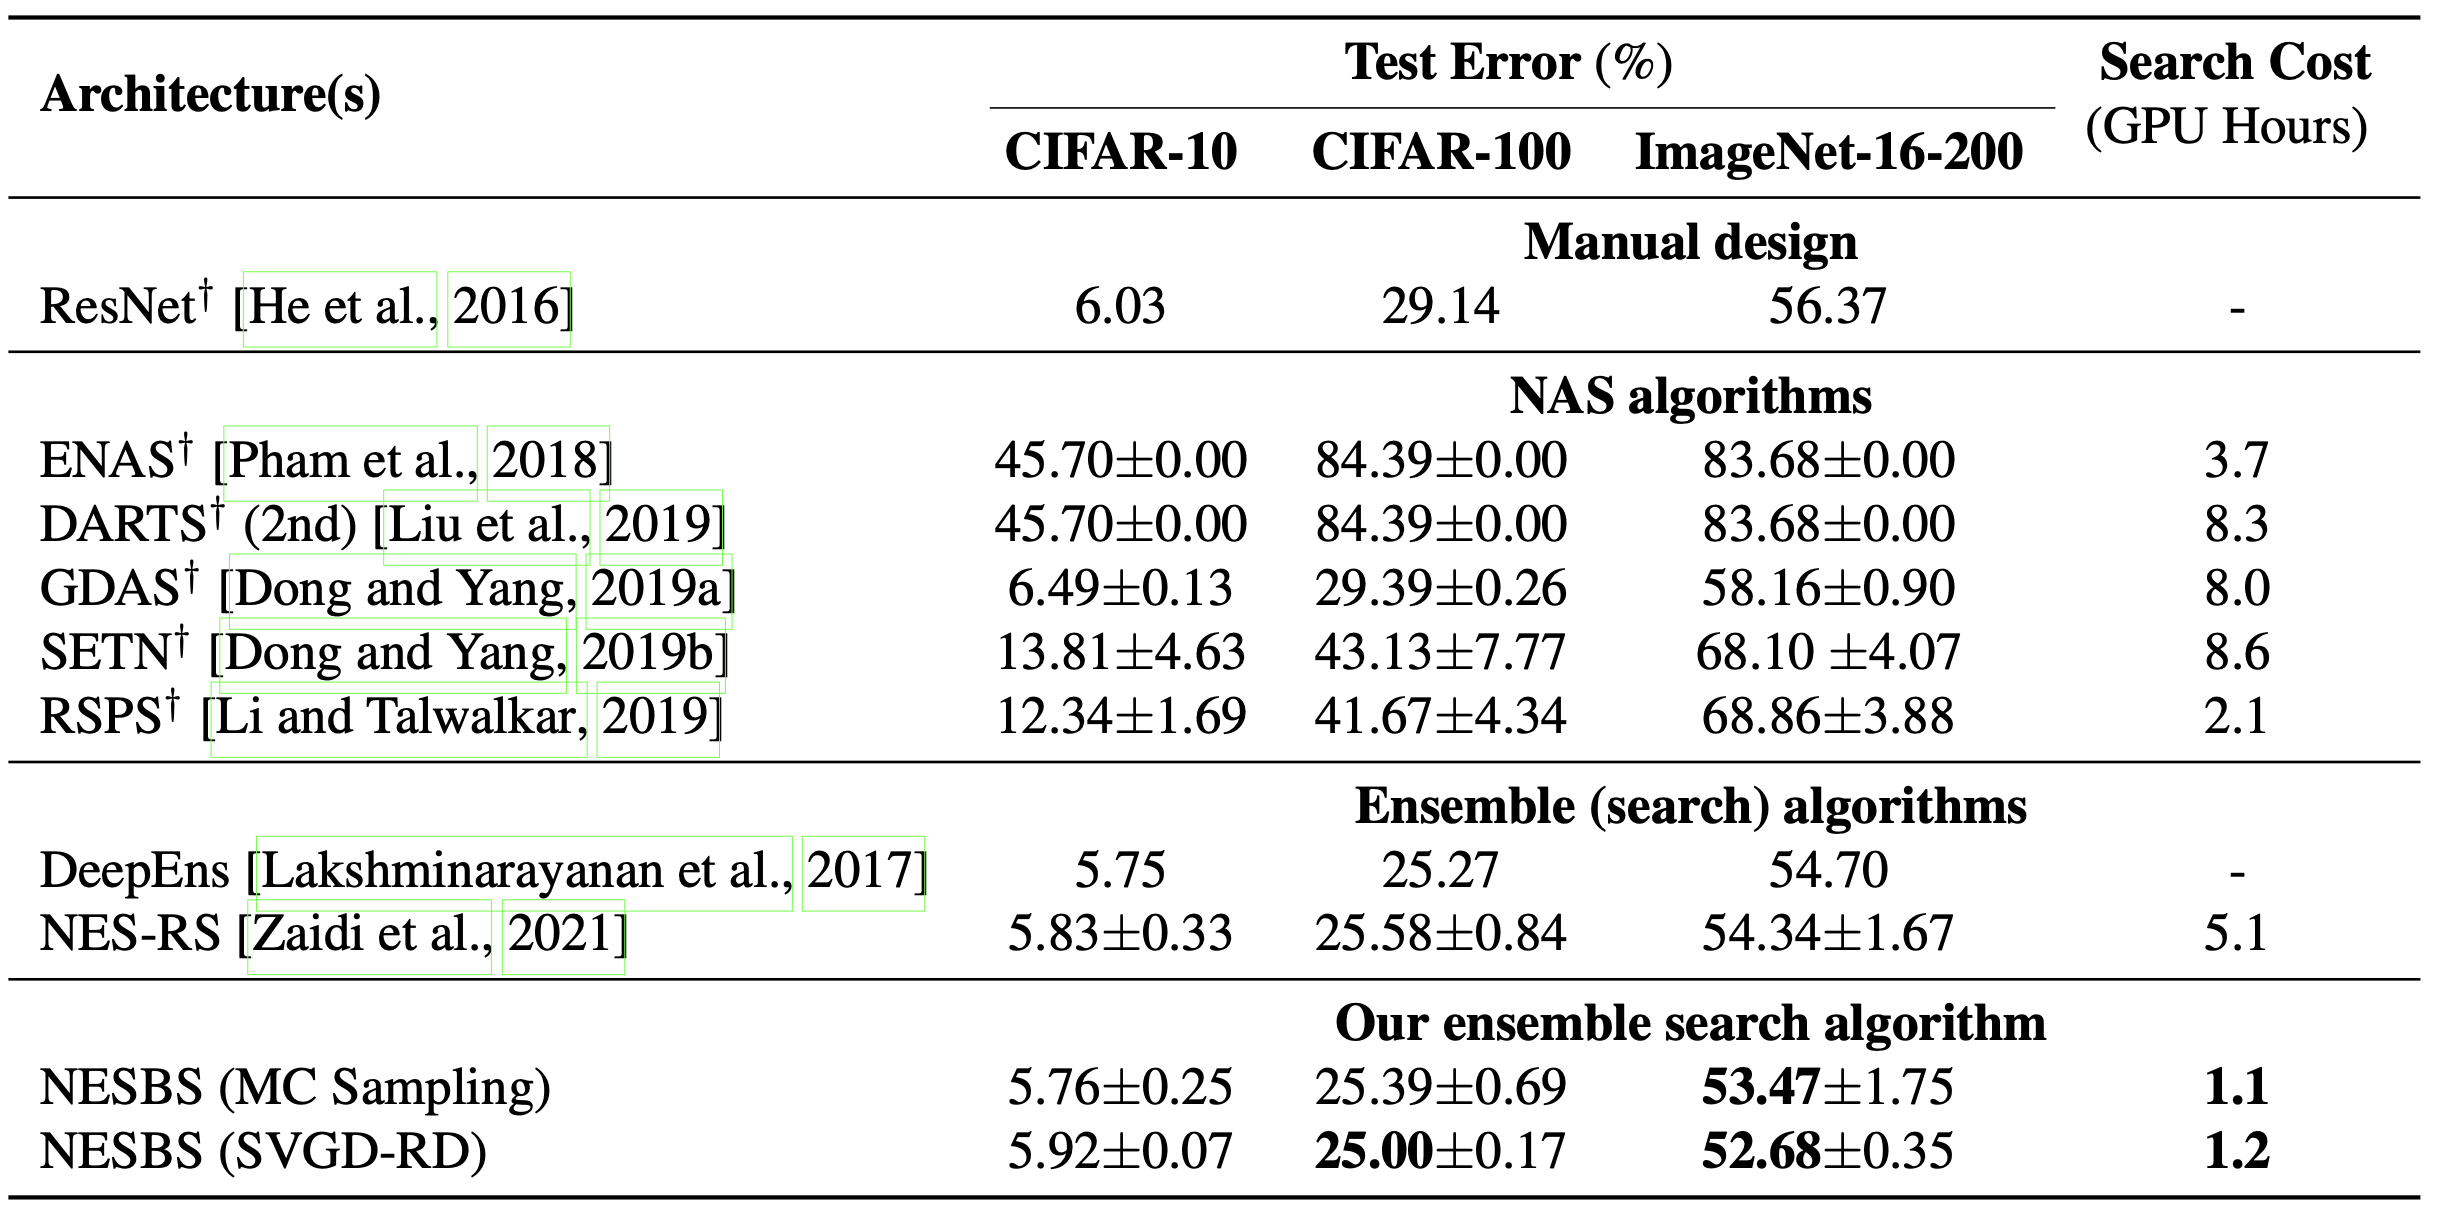
\includegraphics[width=\textwidth]{res1.png}
    \caption{Comparison of architectures selected by different NAS and ensemble (search) algorithms, $n=3$.}
    \label{fig:res1}
\end{figure}
\end{frame}

\begin{frame}{Search in the DARTS space}

\begin{figure}
    \centering
    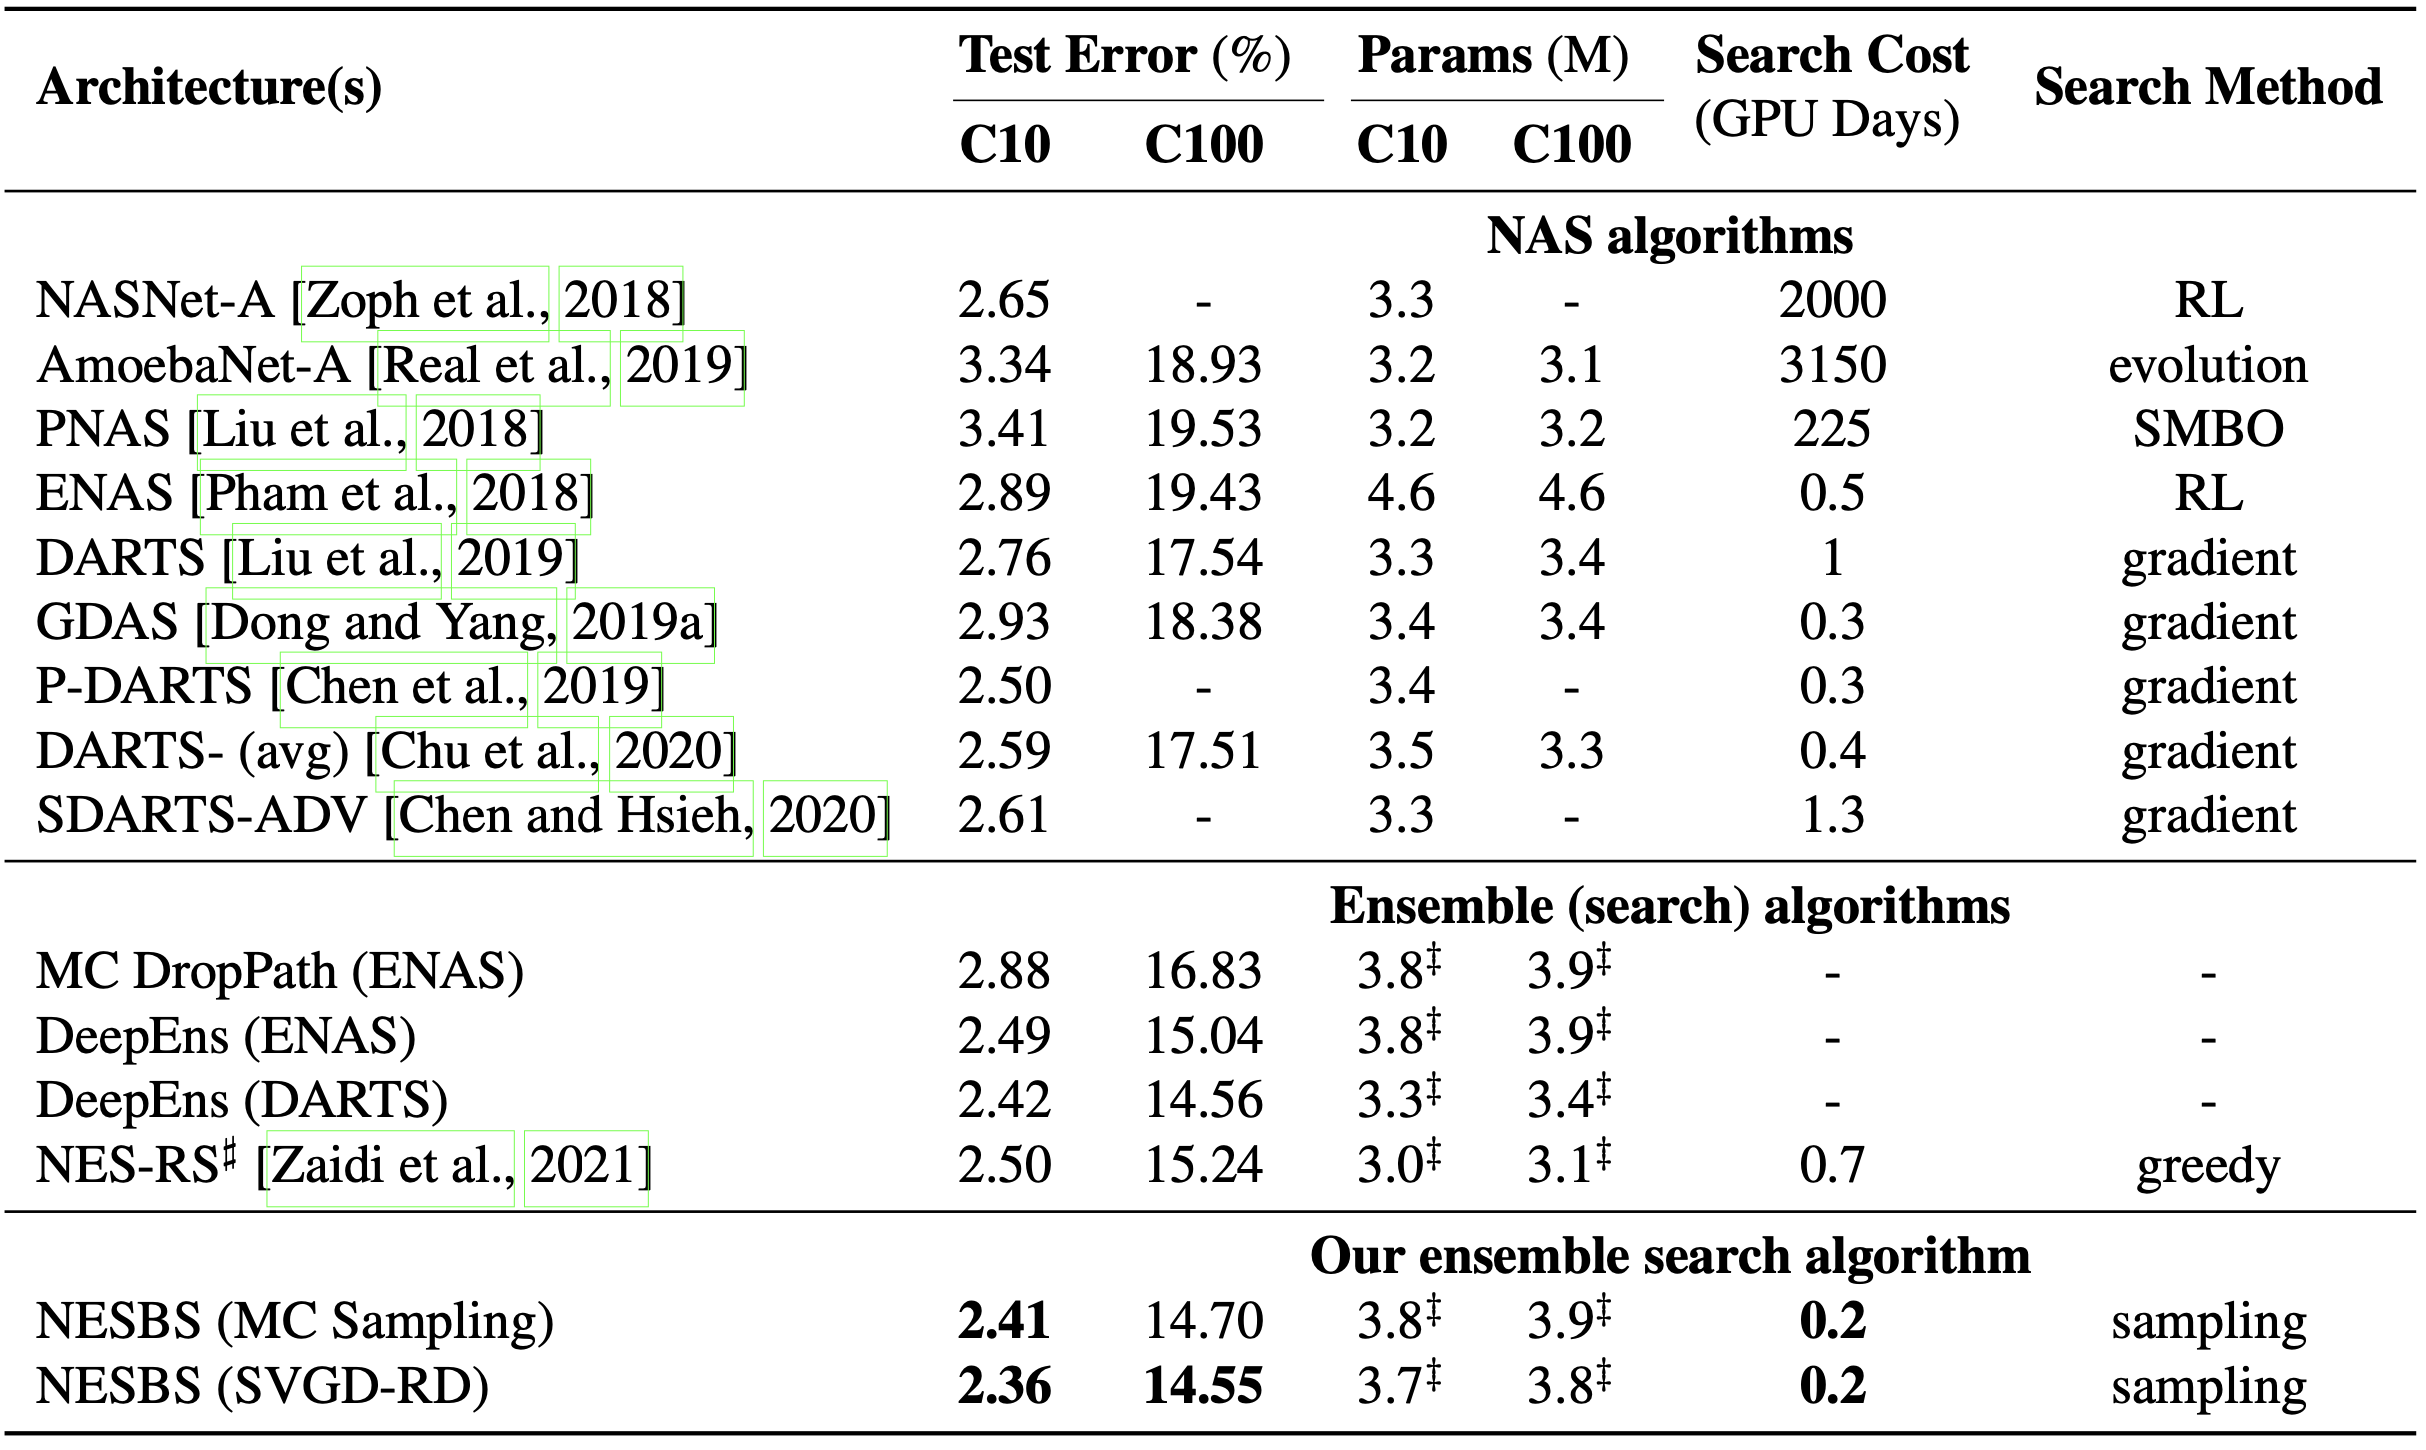
\includegraphics[width=\textwidth]{res2.png}
    \caption{Comparison of different image classifiers on CIFAR-10/100.}
    \label{fig:res2}
\end{figure}

\end{frame}

\begin{frame}{Search in the DARTS space}

\begin{figure}
    \centering
    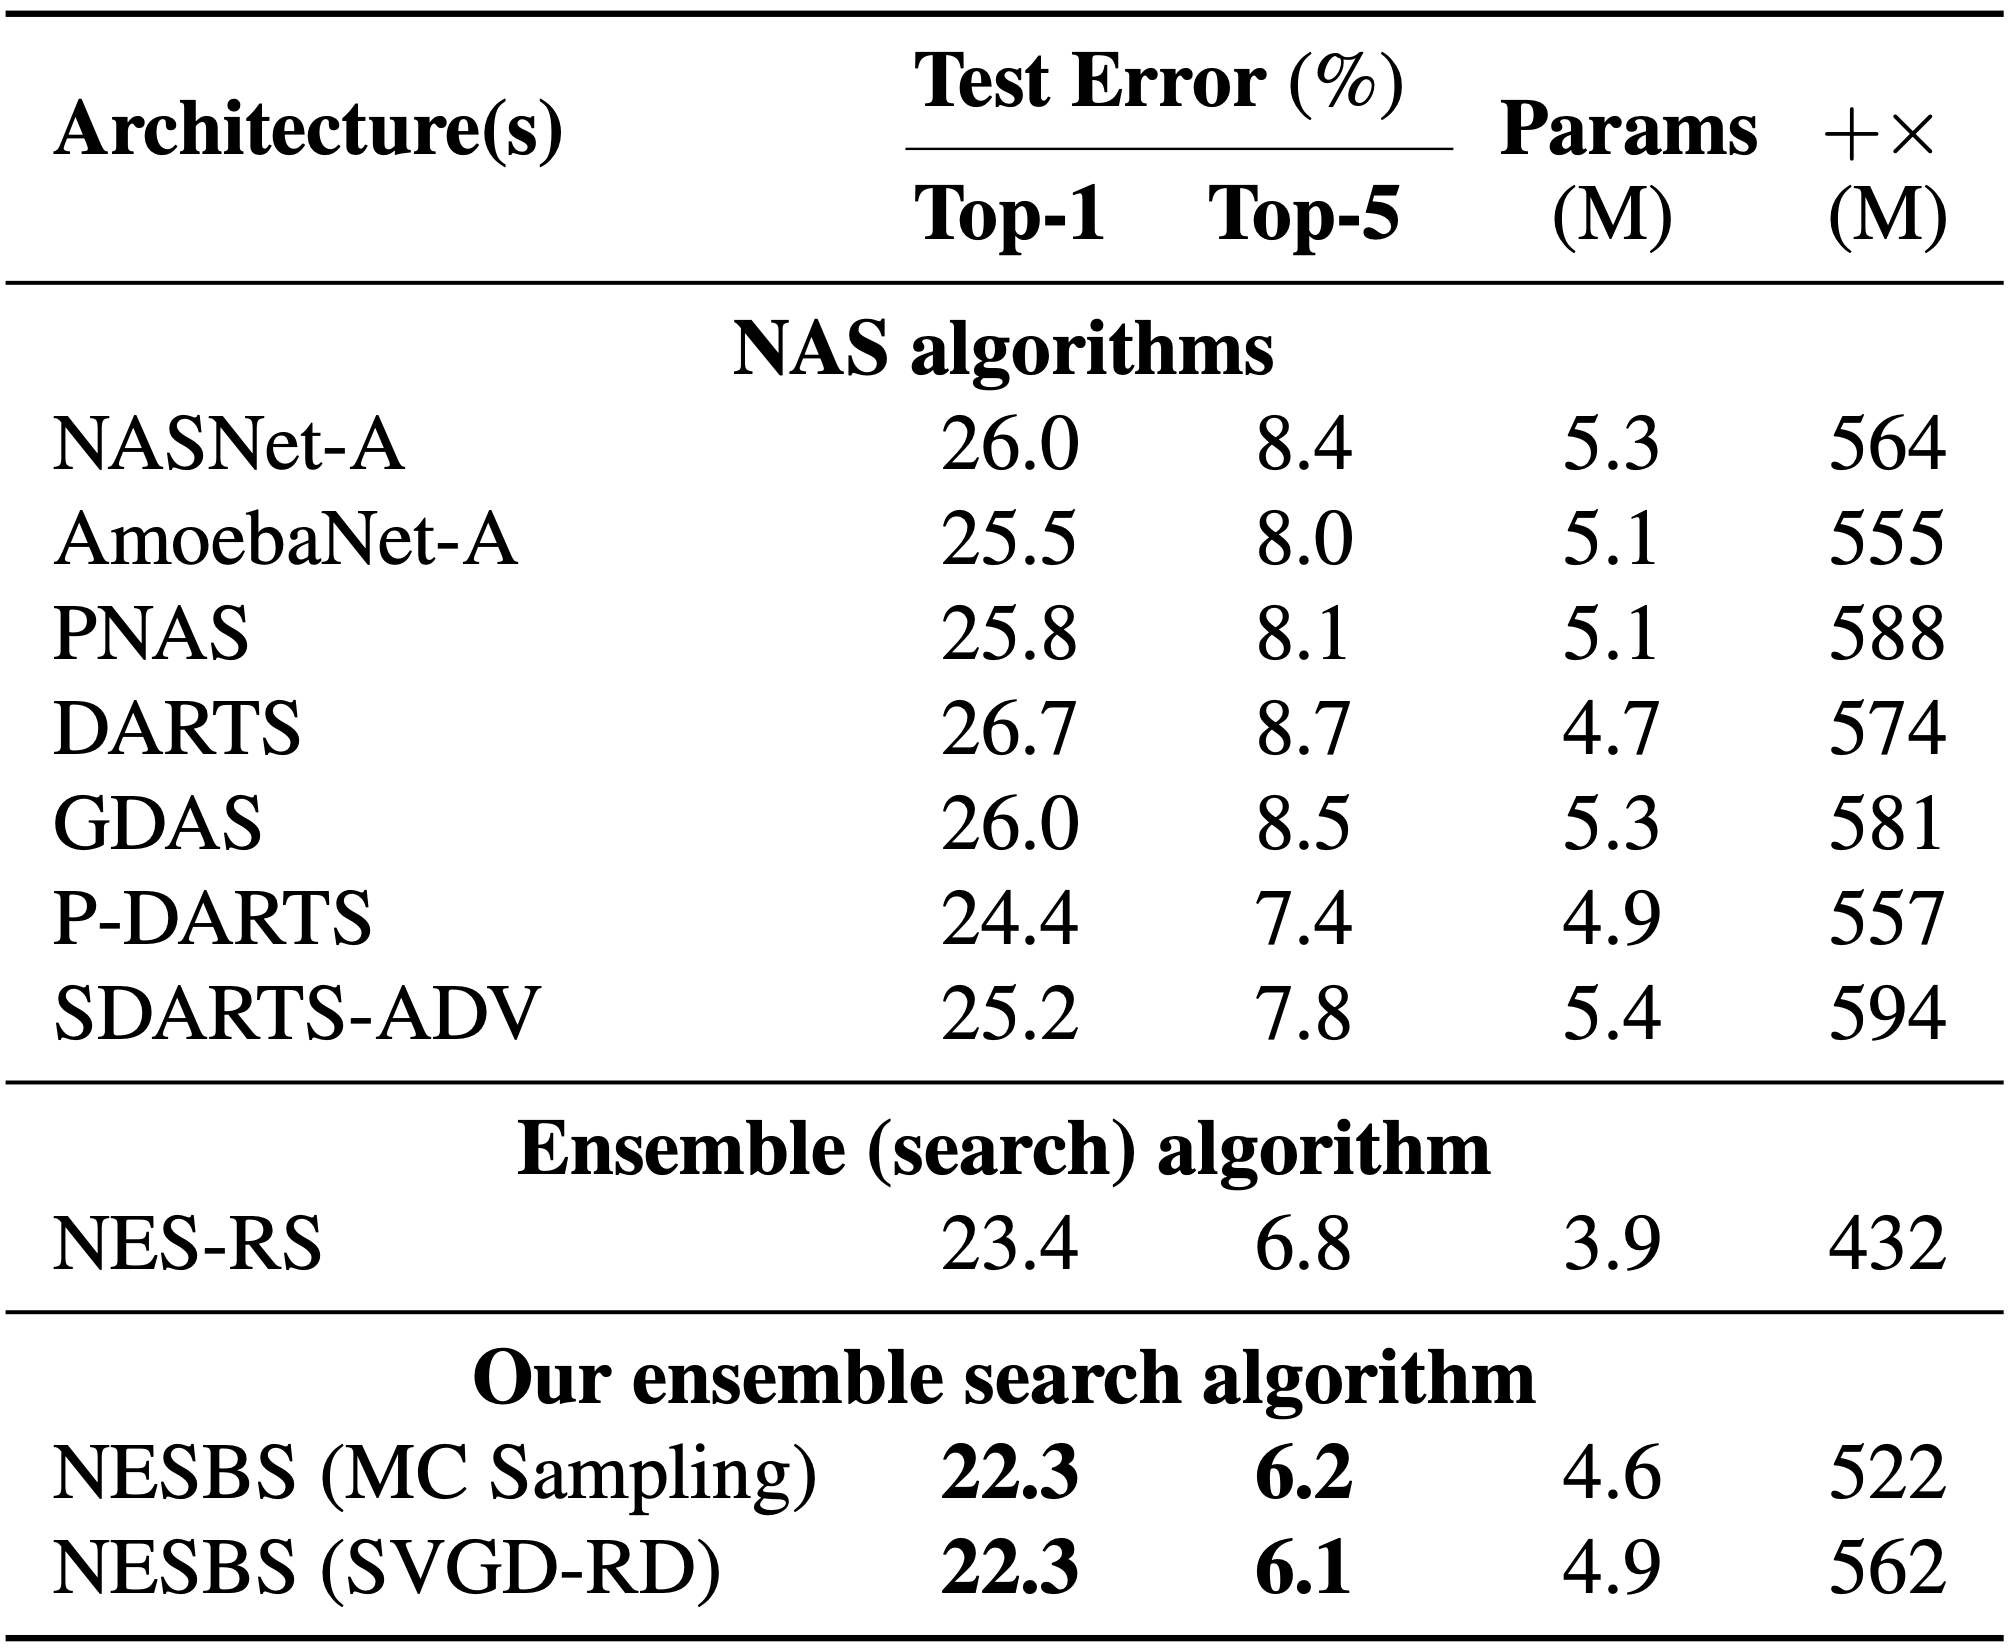
\includegraphics[width=0.7\textwidth]{res3.png}
    \caption{Comparison of image classifiers on ImageNet, $n=3$.}
    \label{fig:res3}
\end{figure}

\end{frame}

\begin{frame}{Search in the DARTS space}

\begin{figure}
    \centering
    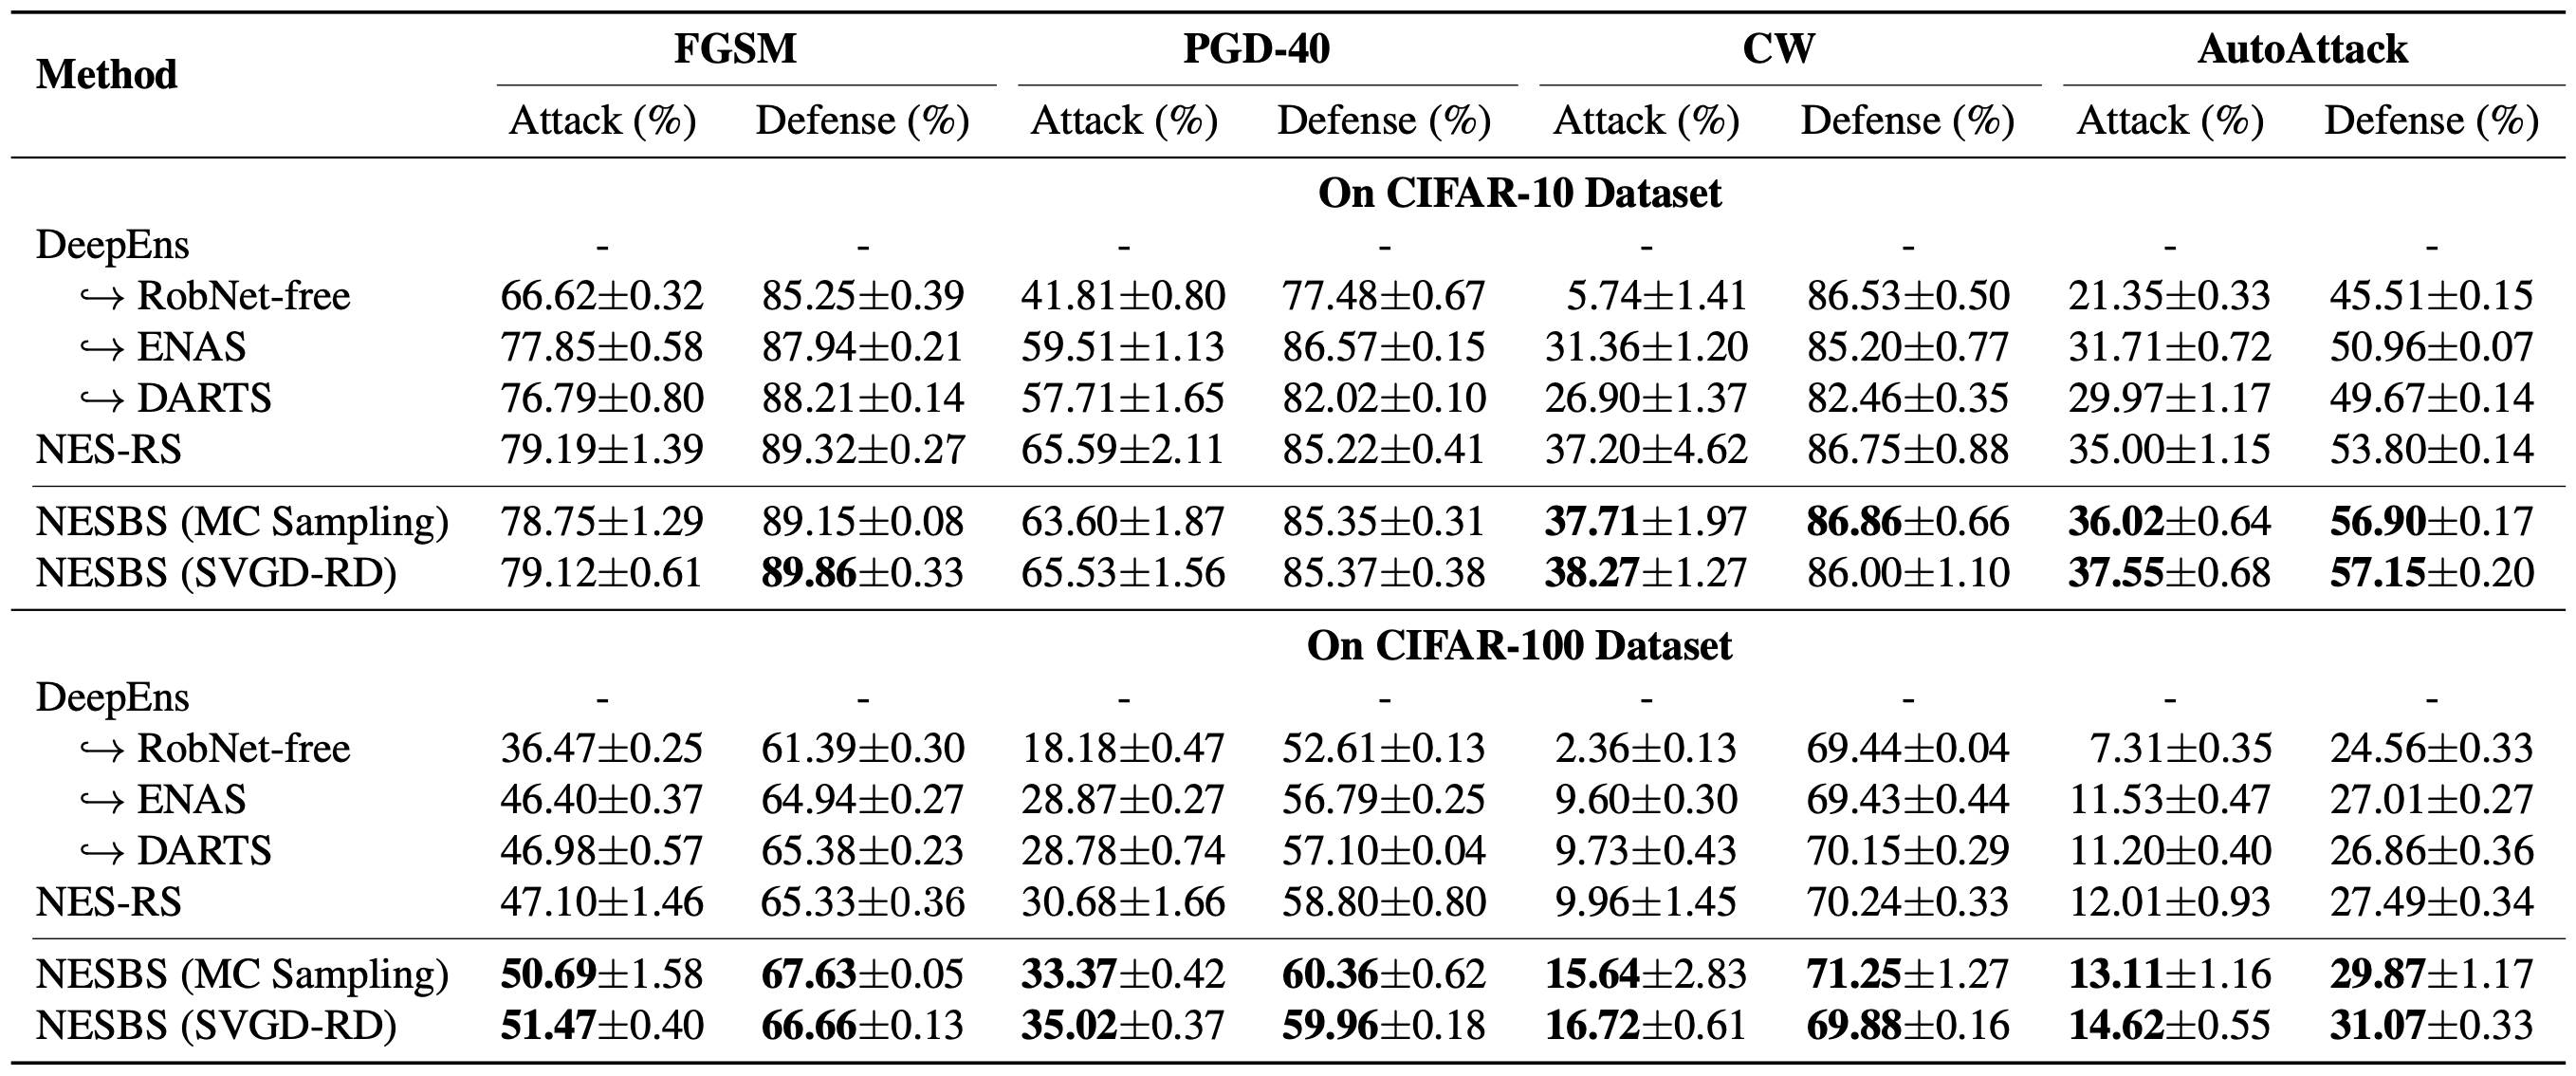
\includegraphics[width=\textwidth]{res4.png}
    \caption{Comparison of adversarial defense among different ensemble (search) algorithms on CIFAR-10/100 under white-box adversarial attacks.}
    \label{fig:res4}
\end{figure}

\end{frame}

\begin{frame}{Single-model performances and diverse model predictions}

\begin{figure}
    \centering
    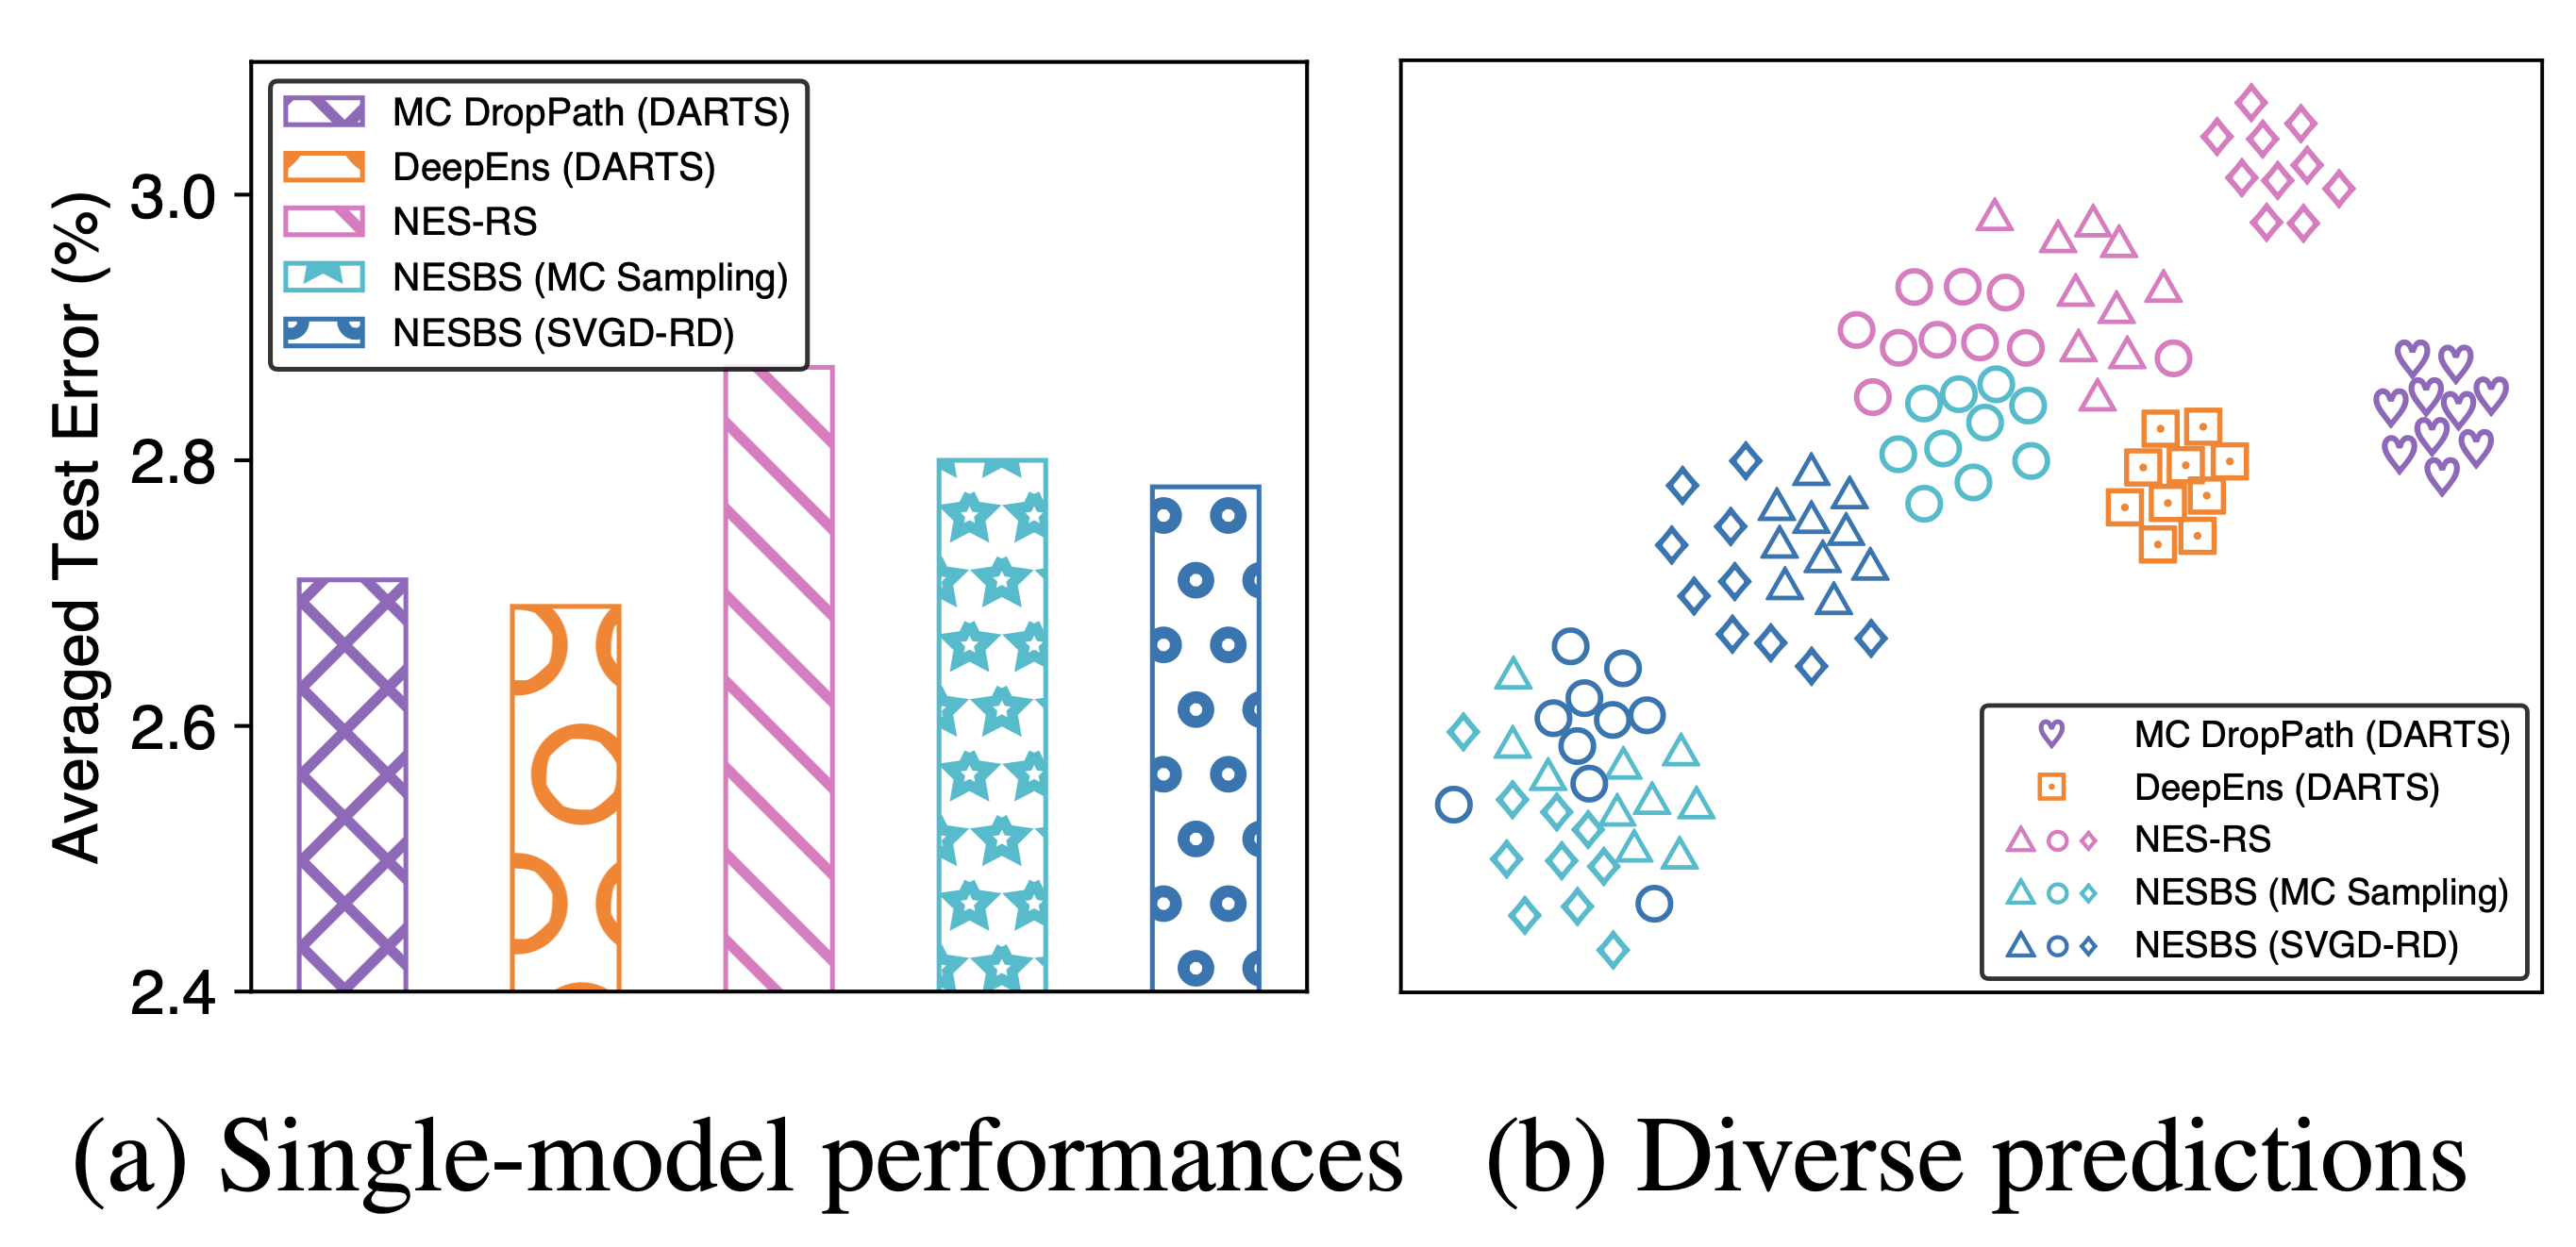
\includegraphics[width=\textwidth]{single_vs_diverse.png}
    \caption{Qualitative comparison of (a) the single-model performances and (b) the diverse model predictions achieved by different ensemble (search) algorithms with an ensemble size of $n = 3$ on CIFAR-10.}
    \label{fig:sin_vs_div}
\end{figure}

\end{frame}

\begin{frame}{Single-model performances and diverse model predictions}

\begin{figure}
    \centering
    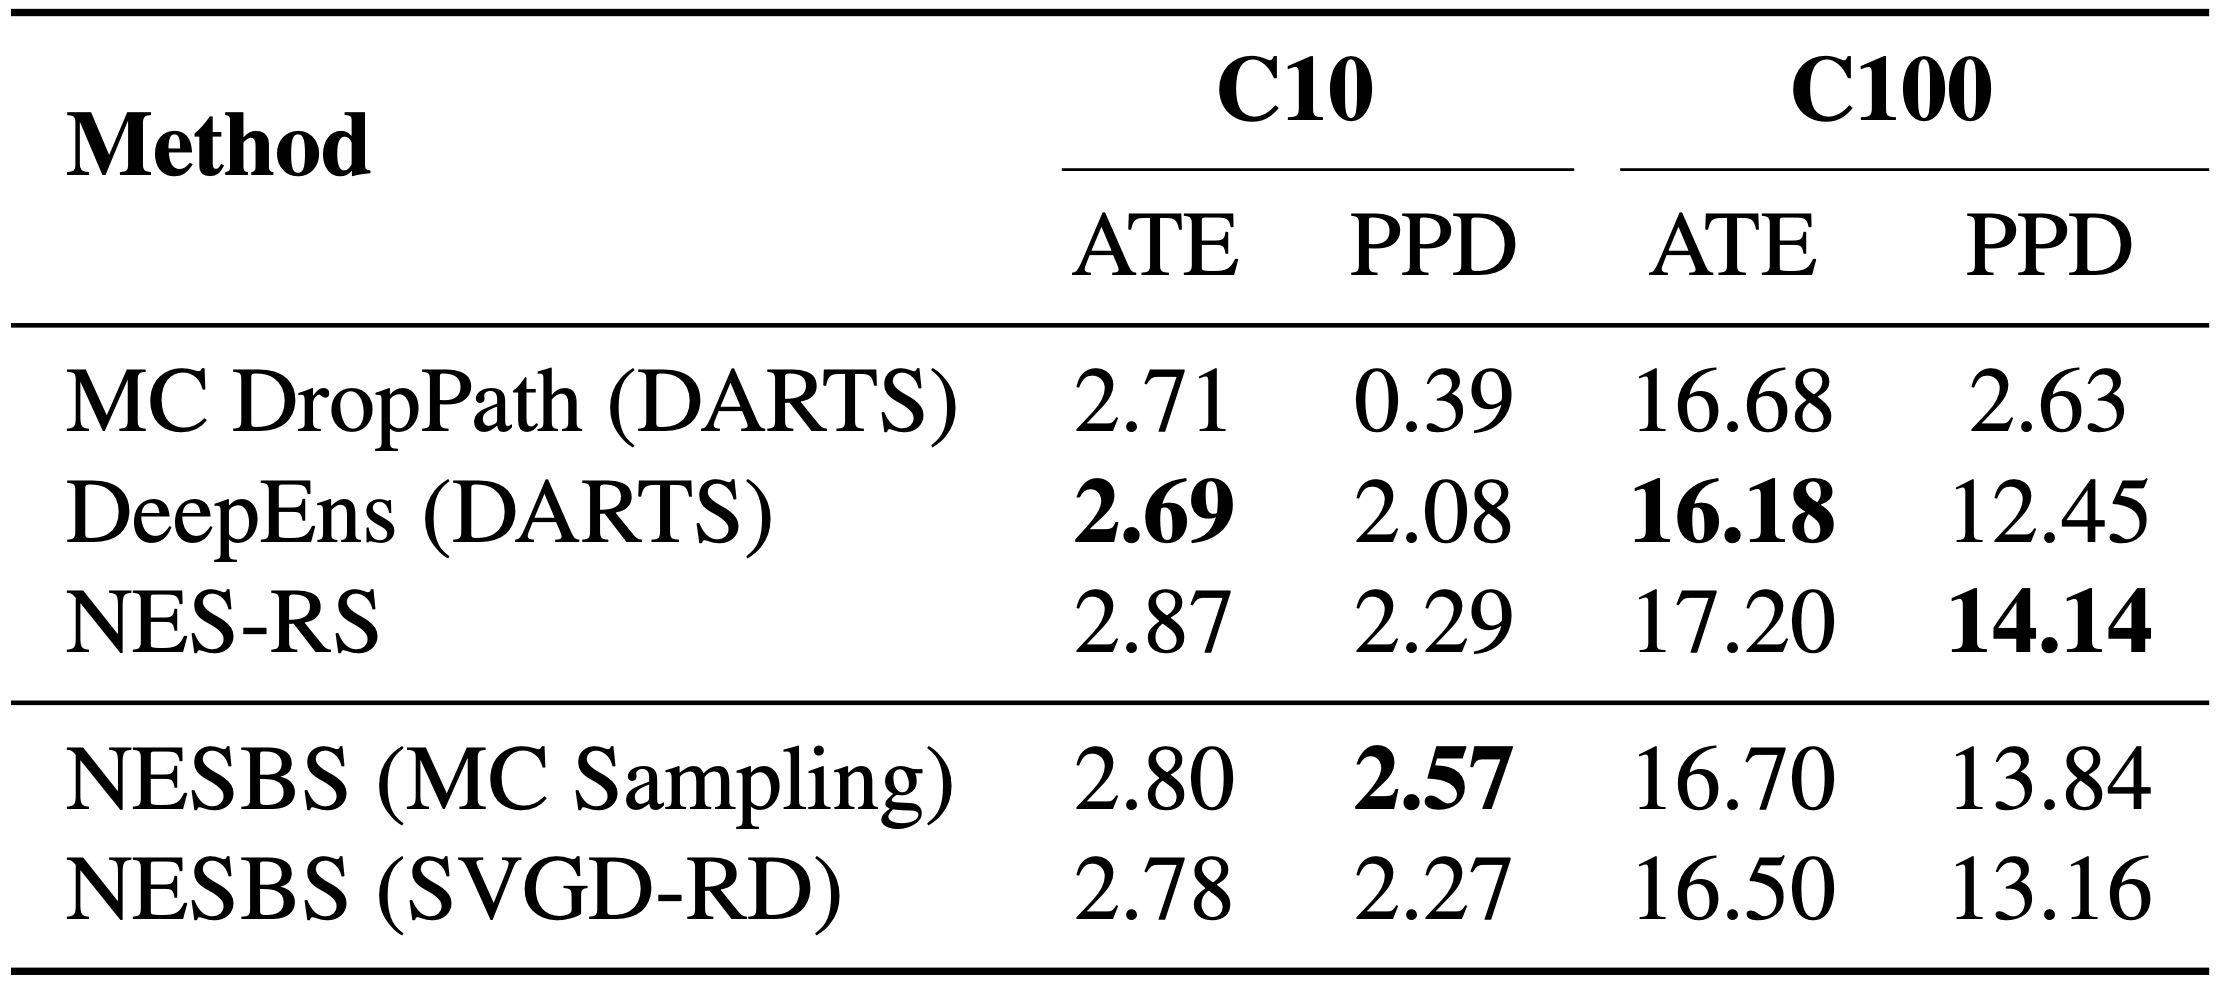
\includegraphics[width=0.9\textwidth]{res5.png}
    \caption{Quantitative comparison of the single-model performances  and the diversity of model predictions achieved by different ensemble (search) algorithms with an ensemble size of 3 on CIFAR-10/100.}
    \label{fig:res5}
\end{figure}

\end{frame}


\begin{frame}{Conclusion}

\begin{itemize}
    \item Novel neural ensemble search algorithms
    \item Effectively and efficiently selects well-performing NNE with diverse architectures from a NAS search space
    \item Achieves improved performances while preserving a comparable search cost
    \item Boosted search effectiveness and efficiency compared to DeepEns and NES-RS
\end{itemize}
\end{frame}


\begin{frame}{Literature}
    \begin{enumerate}
        \item \textbf{Main article} \href{https://proceedings.mlr.press/v180/shu22a/shu22a.pdf}
        {Neural Ensemble Search via Bayesian Sampling}.
    \end{enumerate}
\end{frame}

\end{document}



\documentclass{beamer}
\usepackage{graphicx} % for including images
\usepackage{amsmath, amssymb} % for mathematical formulas

\title{Neural Ensemble Search via Bayesian Sampling}
\subtitle{A Novel Approach to Ensemble Learning in Neural Architectures}
\author{Yao Shu et al.}
\institute{Department of Computer Science, National University of Singapore}
\date{\today}

\begin{document}

\frame{\titlepage}

\begin{frame}
\frametitle{Introduction}
\begin{itemize}
    \item Importance of Neural Architecture Search (NAS) in automating neural network design.
    \item Limitations of traditional NAS focusing on single architectures.
    \item Introduction to Neural Ensemble Search (NES) and its advantages.
\end{itemize}
\end{frame}

\begin{frame}
\frametitle{Related Works}
\begin{itemize}
    \item Overview of existing NAS techniques and their computational costs.
    \item Discussion on neural network ensembles and their historical applications.
    \item Introduction to Stein Variational Gradient Descent (SVGD) and its relevance.
\end{itemize}
\end{frame}

\begin{frame}
\frametitle{Neural Ensemble Search via Bayesian Sampling}
\begin{itemize}
    \item The concept of using Bayesian methods to select diverse, high-performing ensembles.
    \item How the NESBS model estimates ensemble and individual performances.
    \item Overview of Bayesian sampling methods used: MC Sampling and SVGD-RD.
\end{itemize}
\end{frame}

\begin{frame}
\frametitle{Model Training of Supernet}
\begin{itemize}
    \item Explanation of supernet and its role in NESBS.
    \item Methodology for training the supernet to facilitate efficient architecture sampling.
\end{itemize}
\end{frame}

\begin{frame}
\frametitle{Experimental Results}
\begin{itemize}
    \item Performance comparison of NESBS with state-of-the-art NAS methods.
    \item Evaluation metrics and benchmarks used.
    \item Analysis of results showcasing the effectiveness of NESBS.
\end{itemize}
\end{frame}

\begin{frame}
\frametitle{Conclusion and Future Work}
\begin{itemize}
    \item Summary of findings and contributions of the NESBS algorithm.
    \item Discussion on potential improvements and future research directions.
\end{itemize}
\end{frame}

\end{document}